\documentclass{panikzettel}

\title{Effiziente Algorithmen Panikzettel\textsuperscript{\footnotesize TM}}
\author{Luca Oeljeklaus, Christoph von Oy, Tobias Polock, \\Philipp Schröer, Caspar Zecha}
\date{\today}

\usetikzlibrary{arrows.meta}
\usetikzlibrary{decorations.pathmorphing}

%\usepackage{showframe}

\newcommand{\dist}{\mathrm{dist}}
\newcommand{\pot}{\mathrm{pot}}
\newcommand{\rad}{\mathrm{rad}}
\newcommand{\Vin}{V_\text{in}}
\newcommand{\Vout}{V_\text{out}}
\newcommand{\NP}{\mathbf{NP}}
\newcommand{\opt}{\mathrm{opt}}

\newcommand{\nichtrelevant}{\hfill\normalfont\textit{(nicht relevant)}}

\newcommand{\mrhere}[1]{\hyperref[mrExp:#1]{\hypertarget{mr:#1}{\small\sffamily(Hier dein MR)}}}

\begin{document}

\maketitle

\tableofcontents

\section{Einleitung}

Dies ist ein Panikzettel. Doch, doch, du hast richtig gelesen. Wir sind leider auf der Maus ausgerutscht und dabei ist ein kleines Buch entstanden.

Wir haben wieder unnötigen Formalismus weggelassen und Erklärungen so intuitiv gemacht, dass jedes Problem mindestens trivial wirkt.
Zum ersten Mal gibt es auch Beweise, die den Vorhang der Hexerei hinter einigen Algorithmen aufdecken und mit groben Mengen Formalismus untermauern.

Der Panikzettel basiert auf der Vorlesung ``Effiziente Algorithmen'' bei PD Dr.\ Walter Unger im Wintersemester 2017/18.

Aufgrund der unerwarteten Tiefen des Vorlesungsstoffes haben wir in den~\pageref{ende} Seiten noch nicht jede Kleinigkeit erklärt. Daher haben wir \hyperref[sec:merge-requests]{im letzten Kapitel} einige Stellen aufgelistet, an denen du (ja du!) auch selber Hand anlegen kannst.

Dieses Projekt ist lizenziert unter \href{https://creativecommons.org/licenses/by-sa/4.0/}{CC-BY-SA-4.0} und wird auf dem Git-Server der RWTH verwaltet: \url{https://git.rwth-aachen.de/philipp.schroer/panikzettel}.

\newpage
\section{Flussprobleme}

\subsection{Maximum Flow}

\begin{halfboxl}
Bei dem \emph{Flussproblem} versuchen wir den größten Fluss durch Kanten mit Kapazitäten $c$ von einer Quelle $s$ zu seiner Senke $t$ zu senden.

\emph{Mehrere Quellen $S$ / Senken $T$} sind möglich, indem man von den Knoten aus $S$ bzw. $T$ einfach Kanten mit unendlicher (ausreichend großer) Kapazität mit einer \emph{Superquelle} bzw. \emph{Supersenke} verbindet.

\end{halfboxl}%
\begin{halfboxr}
\vspace{-\baselineskip}
\begin{defi}{Flussproblem}
\textbf{Eingabe:} $G = (V,E,s,t,c)$ mit:
\begin{itemize}
    \item $(V,E)$ gerichteter Graph,
    \item $s,t \in V$ und $s \neq t$,
    \item $c : E \to \natplus$
\end{itemize}

\textbf{Ausgabe:} $f : E \in \rnonneg$ mit:
\begin{itemize}
    \item $\Forall e: f(e) \in [0, c(e)]$,
    \item $\Forall v \in V \setminus \Set{s,t}$:\\\footnotesize $\sum_{(a,v) \in E} f((a,v)) = \sum_{(v,a) \in E} f((v,a))$
\end{itemize}

\textbf{Ziel:} Maximiere $w(f) = \sum_{(s,v) \in E} f((s,v))$.
\end{defi}
\end{halfboxr}

\begin{halfboxl}
Das \emph{Restnetzwerk} zu $G$ und $f$ enthält Kanten mit Gewichten entsprechend möglicher Flussveränderung.
Explizit sind auch Rückwärtskanten enthalten, um einen Fluss rückgängig zu machen.

Ein $s$-$t$-Pfad im Restnetzwerk ist immer ein \emph{vergrößernder Pfad}, d.h. über ihn kann man zusätzlichen Fluss schicken.
\end{halfboxl}%
\begin{halfboxr}
\vspace{-\baselineskip}
\begin{defi}{Restnetzwerk}
Zu einem Netzwerk $ = (V, E, s, t, c)$:

Ein \emph{Restnetzwerk} $G_f$ zu einem Fluss $f$ hat Kanten $(v,w) \in V_G^2$ mit Gewicht $\textrm{rest}_f(v,w) > 0$.
\footnotesize
$$\textrm{rest}_f(u,v) := \begin{cases}
    c(u,v) - f(u,v) & \text{falls } (u,v) \in E_G, \\
    f(v,u) & \text{falls } (v,u) \in E_G, \\
    0 & \text{sonst}
\end{cases}$$
\end{defi}
\end{halfboxr}

\subsubsection{Min-Cut Max-Flow}

Ein \emph{Schnitt} $(S,T)$ teilt die Knoten in zwei disjunkte Mengen auf. Die \emph{Kapazität des Schnittes} ist $\sum c(v,w)$ mit $v \in S, w \in T$ (also nur mit Kanten in einer Richtung!).

Für jeden Fluss $f$ und jeden Schnitt $(S,T)$ gilt: $w(f) = f(S,T) \leq c(S,T)$.
\medbreak

\begin{theo}{Min-Cut Max-Flow}
Sei $f$ ein Fluss auf Netzwerk $G = (V,E,s,t,c)$. \par
Dann sind äquivalent:
\begin{enumerate}
    \item $f$ ist maximaler Fluss.
    \item Das Restnetzwerk $G_f$ enthält keinen vergrößernden Pfad.
    \item Es gibt einen Schnitt $(S,T)$ mit $w(f) = c(S,T)$.
\end{enumerate}
\end{theo}
\filbreak

Grobe Beweisideen:
\begin{itemize}
    \item $3 \Rightarrow 1$: Wegen Max-Flow $\leq$ Min-Cut $\leq c(S, T)$  ist $f$ maximal.
    \item $1 \Rightarrow 2$: Wenn es einen vergrößernden Weg geben würde, könnte man $f$ mit diesem vergrößern.
    \item $2 \Rightarrow 3$: Wir teilen den Graphen in von $s$ erreichbare und nicht erreichbare Knoten auf. Per Definition muss dies ein passender Schnitt sein, da es ansonsten noch einen vergrößernden Pfad von $s$ nach $t$ gäbe.
\end{itemize}

\subsubsection{Methode von Ford-Fulkerson, Algorithmus von Edmonds-Karp}

Die \emph{Methode von Ford-Fulkerson} sucht einen maximalen Fluss. Der tatsächliche Algorithmus, einen flussverbessernden Weg in $G_f$ zu finden, bleibt abstrakt. Die Laufzeit ist in $O(C \cdot m_\text{Weg finden})$, wobei $C$ der Wert des maximalen Flusses ist.
Den größten Fluss kann man auch einfach abschätzen mit $C = \sum_{e \in E} c(e)$.

\begin{algo}{Methode von Ford-Fulkerson}
\textbf{Eingabe:} Flussnetzwerk $G = (V, E, s, t, c)$. \\
\textbf{Ausgabe:} Maximaler Fluss $f$.
\tcblower
\begin{enumerate}
    \item Setze $f(e) = 0\quad\Forall e \in E$.
    \item Wiederhole:
        \begin{enumerate}
            \item Bestimme Restnetzwerk $G_f$.
            \item Finde einen flussvergrößernden Weg von $s$ zu $t$ in $G_f$ (BFS/DFS/...).
            \item Gibt es keinen Weg, fertig.
            \item Vergrößere $f$ um den Weg, begrenzt durch den Wert der kleinsten Kante des Weges.
        \end{enumerate}
\end{enumerate}
\end{algo}

Der \emph{Algorithmus von Edmonds-Karp} ist einfach Ford-Fulkerson mit BFS. Laufzeit: $O(m^2 \cdot n) = O(n^5)$.

\begin{itemize}
    \item Zeige, dass $\bigo(m \cdot n)$ Iterationen reichen.
        \begin{itemize}
            \item Zeige $\Forall v \in V: \dist_{G_f^i}(s,v) \leq \dist_{G_f^{i+1}}(s,v))$ für jede Iteration $i$.
                \begin{itemize}
                    \item Gilt für in $G_f^i$ \textbf{gelöschte Kanten}.
                    \item \textbf{Neue Kanten} von $G_f^i$ zu $G_f^{i+1}$ per Induktion: Sei $(v,w)$ eine neue Kante. Sie wurde eingefügt, weil sie vorher als Kante $(w,v)$ auf einem flussvergrößernden Weg lag. Also kann $\dist_{G_f^{i+1}}(s,v)$ nicht kleiner sein als in $G_f^i$. Also gilt $\dist_{G_f^i}(s,v) + 1 = \dist_{G_f^{i+1}}(s,w)$. Weil der Abstand von $w$ zu $s$ sich nicht verbessern kann, gilt die Aussage für jedes $w \in V$.
                \end{itemize}
            \item Wir betrachten Kante $(v,w)$ in Iteration $i$:
                \begin{itemize}
                    \item Falls $(v,w)$ \textbf{gelöscht} wird, so gilt: $\dist_{G_f^i}(s,v) < \dist_{G_f^{i+1}}(s,w)$ (``Flaschenhals'').
                    \item Wenn $(v,w)$ \textbf{wieder eingefügt} wird, gilt $\dist_{G_f^i}(s,w) + 2 \leq \dist_{G_f^{i+1}}(s,w)$, denn wegen Breitensuche war $(v,w)$ auf kürzestem Weg in $G_f^i$.
                \end{itemize}
            \item Wegen $\dist_{G_f^i}(s,t) \leq n - 1$ kann jede Kante höchstens $\floor{(n-1)/2}$ mal gelöscht werden.
            \item In jeder Iteration wird mindestens eine Kante gelöscht.
            \item In jedem $G_f^i$ sind max.\ $2 \cdot m$ Kanten.
            \item Also maximal $\frac{n}{2} \cdot 2 \cdot m = n \cdot m$.
        \end{itemize}
    \item BFS ist in $\bigo(n + m)$.
\end{itemize}

\subsubsection{Algorithmus von Dinitz}

\begin{defi}{Sperrfluss}
In einem Niveaunetzwerk $G'_f = (V, E_f',s,t,c')$ und mit Fluss $f'$ auf $G'$:
\begin{itemize}
    \item Eine Kante $e \in E_f'$ ist \emph{saturiert}, falls $f'(e) = rest_f(e)$.
    \item $f'$ heißt \emph{Sperrfluss}, falls jeder Weg von $s$ nach $t$ in $G_f'$ eine saturierte Kante hat.
    \item Ein Knoten $v$ heißt \emph{saturiert}, falls $\pot(v) = 0$ mit: \\
    $\pot(v) := \min \Set{\sum_{e \in N_\text{in}(v)} rest_f(e), \sum_{e \in N_\text{out}(v)} rest_f(e)}$
\end{itemize}
\end{defi}

\begin{halfboxl}
Die Idee: Suche gleich mehrere verbessernde Wege in $G_f$.
Dies machen wir in einem \emph{Niveaunetzwerk}, einem Restnetzwerk in dem es nur Kanten zwischen benachbarten Schichten gibt, d.h. nur Kanten zwischen Knoten mit unterschiedlicher Distanz zu $s$.
Darin bestimmen wir einen Sperrfluss.

Die Anzahl der Iterationen ist maximal $n-1$: In jedem Schritt $i$ werden alle Wege der Länge $l_i = \dist_{G_f'}(s,t)$ getrennt. Neu entstehende Kanten führten vorher von Schicht $i$ zu $i-1$, damit müssen neue Wege mindestens Länge $l_i+2$ haben.
\end{halfboxl}%
\begin{halfboxr}
\vspace{-\baselineskip}
\begin{algo}{Dinitz}
\textbf{Eingabe:} Flussnetzwerk $G = (V, E, s, t, c)$. \\
\textbf{Ausgabe:} Maximaler Fluss $f$.
\tcblower
\begin{enumerate}[nosep]
    \item Setze $f(e) = 0\quad\forall e \in E$.
    \item Wiederhole:
        \begin{enumerate}[nosep]
            \item Bestimme Restnetzwerk $G_f$.
            \item Bestimme Niveaunetzwerk $G_f'$.
            \item Bestimme Sperrfluss $f'$ in $G_f'$.
            \item Falls $w(f') = 0$, fertig.
            \item Sonst erweitere $f$ um $f'$.
        \end{enumerate}
\end{enumerate}
\end{algo}
\end{halfboxr}

\begin{halfboxl}
Ein Sperrfluss kann in $\bigo(n^2)$ mit wiederholter \emph{Forward-Backward-Propagation} bestimmt werden.

\emph{Forward Propagation}: Knotenpotentiale $\pot(v)$ vorwärts durch das Niveaunetzwerk schieben, beginnend vom Knoten mit kleinstem Potential. \emph{Backward Propagation} ist analog: Statt $\Vout(v)$ $\Vin(v)$ verwenden. Eine \emph{Propagationsphase} führt Forward und Backward Propagation aus.

Jede Propagationsphase läuft in $\bigo(n+l_i)$ mit $l_i$ Anzahl neu saturierter Kanten. Nach maximal $n-1$ Propagationsphasen ist ein Sperrfluss gefunden. Also Laufzeit für die iterierte Propagation: $\bigo(\sum_{i=1}^{n-1} (n+l_i)) = \bigo(n^2 + m)$.
\end{halfboxl}%
\begin{halfboxr}
\vspace{-\baselineskip}
\begin{algo}{Iterierte Propagation}
\textbf{Eingabe:} $G'_f = (V, E'_f, s, t, c')$. \\
\textbf{Ausgabe:} Sperrfluss $f'$.
\tcblower
Solange kein Sperrfluss $f'$ berechnet ist, wiederhole:
\begin{enumerate}
    \item Führe eine \emph{Propagationsphase} aus: \\
          Forward, dann Backward Propagation.
    \item Entferne alle saturierten Kanten und Knoten.
\end{enumerate}
\end{algo}
\end{halfboxr}

\begin{algo}{Forward Propagation bzw. Backward Propagation}
\textbf{Eingabe:} Niveaunetzwerk $G'_f = (V, E'_f, s, t, c')$. \\
\textbf{Ausgabe:} Neuer Fluss $f''$. \\
\emph{(Verwende $\Vin$ für Backward Propagation)}
\tcblower
\begin{enumerate}[nosep]
    \item Setze $f(e) = 0\quad\Forall e \in E$.
    \item Wiederhole:
        \begin{enumerate}[nosep]
            \item Bestimme $v = \min_{v \in V, \pot(v) > 0} \pot(v)$.
            \item Setze $U(v) = \pot(v)$ und sonst $U(w) = 0$.
            \item $v$ in neue Schlange $Q$.
            \item Solange (neues) $v$ aus $Q$ entnehmbar ist, für jedes $e = (v,w) \in \Vout(v)$:
                \begin{enumerate}[nosep]
                    \item $f''(e) = \min \Set{\pot(e), U(v)}$.
                    \item $U(v) = U(v) - f''(e)$.
                    \item $U(w) = U(w) + f''(e)$.
                    \item Falls $w \neq t$ und $U(w) = f''(e)$, füge $w$ in $Q$ ein.
                \end{enumerate}
        \end{enumerate}
\end{enumerate}
\end{algo}

\begin{bonus}{BFS, DFS, ...}
Die Propagation verwendet eine Schlange $Q$, also BFS. DFS wäre aber ebenso möglich, hat u.U.\ schlechtere Laufzeit.
\end{bonus}

\subsection{Mindestfluss}

\begin{halfboxl}
Bei dem \emph{Mindestflussproblem} versuchen wir den größten Fluss durch Kanten mit Kapazitäten $c$ von einer Quelle $s$ zu seiner Senke $t$ zu senden. Dazu besitzt jede Kante eine untere Schranke $c'$ die den kleinsten Fluss darstellt, der mindestens durch diese Kante fließen muss.

Es ist außerdem am folgenden Beispiel festzustellen, dass es nicht immer eine Lösung gibt:
\begin{center}
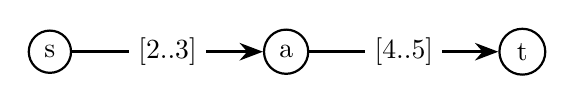
\begin{tikzpicture}[every node/.style={circle,thick,draw},
              >={Stealth[black]},
              every edge/.style={draw=black,very thick,
              every node/.style={fill=white}}]
    \node (s) at (0,0) {s};
    \node (a) at (3,0) {a};
    \node (t) at (6,0) {t};

    \path [->] (s) edge node {$[2 .. 3]$} (a);
    \path [->] (a) edge node {$[4 .. 5]$} (t);
\end{tikzpicture}
\end{center}

\end{halfboxl}%
\begin{halfboxr}
\vspace{-\baselineskip}
\begin{defi}{Mindestflussproblem}
\textbf{Eingabe:} Ein Graph analog zum Flussproblem, zusätzlich:
\begin{itemize}[nosep]
    \item $c' : E \to \natplus$
\end{itemize}

\textbf{Ausgabe:} $f : E \in \rnonneg$ analog zum Flussnetzwerk, zusätzlich:
\begin{itemize}[nosep]
    \item $\Forall e: c'(e) \le f(e) \le c(e)$
\end{itemize}

\textbf{Ziel:} Bestimme, ob eine solcher Fluss existiert. Falls ja, maximiere: \begin{tightcenter}$w(f) = \sum\limits_{(s,v) \in E} f((s,v))$\end{tightcenter}
\end{defi}
\end{halfboxr}

\begin{tightcenter}
\begin{tikzpicture}[every node/.style={circle,thick,draw},
            >={Stealth[black]},
            every edge/.style={draw=black,very thick, every node/.style={fill=white}}]
    \node[ultra thick] (s) {s};
    \node[right = 1.5 of s] (a)  {a};
    \node[right = 3 of a] (b) {b};
    \node[ultra thick, right = 1.5 of b] (t) {t};

    \path [->,decoration={snake,amplitude=.4mm,segment length=2mm,post length=1mm}] (s) edge[decorate,thick] (a);
    \path [->] (a) edge[draw=reddishpurple,ultra thick] node {$[u .. o]$} (b);
    \path [->,decoration={snake,amplitude=.4mm,segment length=2mm,post length=1mm}] (b) edge[decorate,thick] (t);
\end{tikzpicture}

\begin{tikzpicture}[every node/.style={circle,thick,draw},
              >={Stealth[black]},
              every edge/.style={every node/.style={fill=white}, draw=black,very thick}]
    \node (s) {s};
    \node[right = 1.5 of s] (a) {a};
    \node[right = 1.5 of a] (x) {x};
    \node[right = 1.5 of x] (y) {y};
    \node[right = 1.5 of y] (b) {b};
    \node[right = 1.5 of b] (t) {t};
    \node[ultra thick, above left = 1 and 1 of s] (s') {s'};
    \node[ultra thick, below right = 1 and 1 of t] (t') {t'};

    \path [->,decoration={snake,amplitude=.4mm,segment length=2mm,post length=1mm}] (s) edge[decorate,thick] (a);
    \path [->] (a) edge[draw=reddishpurple,ultra thick] node {$o$} (x);
    \path [->] (x) edge[draw=reddishpurple,ultra thick] node {$o-u$} (y);
    \path [->] (y) edge[draw=reddishpurple,ultra thick] node {$o$} (b);
    \path [->,decoration={snake,amplitude=.4mm,segment length=2mm,post length=1mm}] (b) edge[decorate,thick] (t);
    \path [->] (s') edge[draw=bluishgreen, bend left = 10] node {$u$} (y);
    \path [->] (x) edge[draw=bluishgreen, bend right = 10] node {$u$} (t');
    \path [->] (s') edge[draw=bluishgreen] node[below left, fill=none] {$\sum\limits_{e \in E}c(e)$} (s);
    \path [->] (t) edge[draw=bluishgreen] node[above right, fill=none] {$\sum\limits_{e \in E}c(e)$} (t');
\end{tikzpicture}
\end{tightcenter}

\begin{halfboxl}
Wir können das Problem mit einer effizienten Reduktion auf das normale Flussproblem lösen.

Dafür wandeln wir mit dem nebenstehenden Algorithmus ein Netzwerk $G$ mit Mindesfluss in ein Netzwerk $G'$ um.

Wenn dann in $G$ gilt $u \leq f(a,b) \leq o$, dann gibt es einen Fluss $f'$ in $G'$, sodass gilt:
\begin{alignat*}{2}
    f'(s',y) &= f'(x,t') &&= u \\
    f'(a,x) &= f'(y,b) &&= f(a,b) \\
    f'(x,y) & &&=f(a,b) - u
\end{alignat*}

Andersherum können wir von einem korrekten Fluss in $G'$ wieder zu einem Fluss in $G$ kommen.
Wenn alle Kanten $(s',y)$ und $(x,t')$ saturiert sind, gilt $f'(a,x) = f'(y,b)$ und damit auch:
\[ f(a,b) = f'(a,x) \]

Oder anders gefragt: Was wäre, wenn $f(a,b) < u$ in $G$? Dann ist in $G'$ mindestens $s \rightsquigarrow a$ oder $b \rightsquigarrow t$ begrenzend. Also kann $(s',y)$ oder $(x,t')$ nicht saturiert werden.
\end{halfboxl}%
\begin{halfboxr}
\vspace{-\baselineskip}
\begin{algo}{Reduktion des Mindestflussproblems auf das Flussproblem}
\textbf{Eingabe:} $G = (V, E, s, t, c, c')$ \\
\textbf{Ausgabe:} $G' = (V', E', s', t', c'')$.
\tcblower
\begin{enumerate}[nosep]
    \item Füge neue Quelle und Senke $s'$ und $t'$ ein.
    \item Ersetze jede Kante $(a,b)$ durch drei Kanten $(a,x)$, $(x,y)$ und $(y,b)$.
    \item Erzeuge Kanten $(s',y)$ und $(x,t')$.
    \item Setze Kantengewichte:
        \begin{alignat*}{2}
            c''(a,x) &= c''(y,b) &&:= c(a,b) \\
            c''(x,y) & &&:= c(a,b) - c'(a,b) \\
            c''(s', y) &= c''(x, t') &&:= c'(a,b) \\
            c''(t,t') &= c''(s',s) &&:= \sum\limits_{e \in E} c(e)
        \end{alignat*}
\end{enumerate}
\end{algo}
\end{halfboxr}

\subsection[Flüsse mit Alternativen]{Flüsse mit Alternativen\nichtrelevant}

Man könnte das Mindestflussproblem so erweitern, dass ein Fluss über eine Kante $e$ nicht nur in $[c(e), c'(e)]$ liegen muss, sondern alternativ auch gleich null sein kann.

Bäm, schon ist das Problem $\NP$-schwer. Dies kann man mit einer Reduktion von Exakt-3-SAT zeigen.

\subsection{Min-Cost-Flow}

\begin{halfboxl}
Beim \emph{Min-Cost-Flow-Problem} wird nach einem Fluss mit exaktem Betrag $W$ gesucht, der Kosten minimiert. Die Kosten einer Kante sind dabei proportional zum Fluss, der durch sie fließt.

Wenn $W = 1$, dann haben wir das Problem des kürzesten Weges.

\end{halfboxl}%
\begin{halfboxr}
\vspace{-\baselineskip}
\begin{defi}{Min-Cost-Flow-Problem}
Genau wie das normale Flussproblem, aber zusätzlich:

\textbf{Eingabe:} $l : E \to \nat$ und $W \in \nat$

\textbf{Ziel:} Bestimme Fluss $f$ mit $w(f) = W$ und minimalem $l(f) = \sum\limits_{e \in E} f(e) \cdot l(e)$.
\end{defi}
\end{halfboxr}
\begin{halfboxl}
Für den Algorithmus brachen wir den Begriff des \emph{Kreisflusses}:

Ein Fluss $f'$ ist ein \emph{Kreisfluss} gdw.\\ $\Forall v \in V: f'_\text{in}(v) = f'_\text{out}(v)$.

Zum Algorithmus.

In jedem Kreisfluss $f'$ gilt $w(f') = 0$. Wir können also durch Kreise Kosten verbessern, ohne den Flusswert zu ändern. Dies geht immer, bis $f$ kostenminimal ist.

Wenn $l(e) = 0~\Forall e \in E$, dann muss nur ein Fluss mit $w(f) = W$ gefunden werden.
\end{halfboxl}%
\begin{halfboxr}
\vspace{-\baselineskip}
\begin{algo}{Min-Cost-Flow}
\textbf{Eingabe:} $G = (V, E, s, t, c, l)$, $W \in \nat$. \\
\textbf{Ausgabe:} Fluss $f$ mit $w(f) = W$.
\tcblower
\begin{enumerate}
    \item Bestimme beliebigen Fluss $f$ mit $w(f) = W$.
    \item Verbessere die Kosten:
        \begin{itemize}
            \item Solange es in $G_f$ einen Kreis $C$ mit negativen Kosten gibt:
                \begin{itemize}
                    \item[] $f = f + f'$
                \end{itemize}
        \end{itemize}
\end{enumerate}
\end{algo}
\end{halfboxr}
\medbreak

\begin{halfboxl}
\begin{proof}
Es gelte $l(f^\ast) < l(f)$ für einen besseren Fluss $f^\ast$.
Sei dann $f'(e) := f^\ast(e) - f(e)~\Forall e \in E$.

$f'$ ist dann zyklisch, weil $f^\ast$ und $f$ zur Quelle und Senke gleichen Fluss haben müssen.

$f'$ besteht aus $m' < m$ Kreisflüssen $f'_i$.
Also: $l(f') = l(f^\ast) - l(f) = \sum_{i=1}^{m'} l(f'_i)$.
Wegen $l(f^\ast) < l(f)$ muss es ein $j$ mit $l(f'_j) < 0$ geben.
\end{proof}
\end{halfboxl}%
\begin{halfboxr}
\vspace{-\baselineskip}
\begin{theo}{Kostenminimalität}
Falls $f$ nicht kostenminimal ist, dann gibt es einen Kreis $C$ in $G_f$, auf dem $f$ negative Kosten hat.
\end{theo}
\end{halfboxr}

\begin{halfboxl}
Wir können den Algorithmus schneller machen, indem wir ``bessere'' Kreise bevorzugt wählen.
Mit dem Min-Mean-Cycle-Algorithmus kommen wir so insgesamt auf eine bessere Laufzeit.
Genauer wollen wir Kreise so wählen, dass die durchschnittlichen Kantenkosten $\overline{l}(C)$ eines Kreises $C$ minimiert werden:
\[
  \overline{l}(C) = \frac{\sum_{e \in C} l(e)}{\abs{C}}
\]

Der Algorithmus läuft in $\bigo(m^3 \cdot n^2 \cdot \log n) \cap \bigo(m^2 \cdot n^2 \cdot \log(nL))$, dabei wird $\bigo(m^2 \cdot n \cdot \log n) \cap \bigo(m \cdot n \cdot \log(nL))$ oft ein Min-Mean-Cycle gesucht. \mrhere{mean-algo}
\end{halfboxl}%
\begin{halfboxr}
\vspace{-\baselineskip}
\begin{algo}{Mean-Algorithmus}
\textbf{Eingabe:} $G = (V, E, s, t, c, l)$, $W \in \nat$. \\
\textbf{Ausgabe:} Fluss $f$ mit $w(f) = W$.
\tcblower
\begin{enumerate}
    \item Bestimme beliebigen Fluss $f$ mit $w(f) = W$.
    \item Verbessere die Kosten:
        \begin{itemize}
            \item Solange es in $G_f$ einen Kreis $C$ mit negativen Kosten gibt:
                \begin{enumerate}
                    \item Setze $C = \hyperref[algo:min-mean-cycle]{min-mean-cycle} (V)$
                    \item Bestimme maximalen zyklischen Fluss $f'$ auf $C$.
                    \item $f = f + f'$.
                \end{enumerate}
        \end{itemize}
\end{enumerate}
\end{algo}
\end{halfboxr}

Für den Laufzeitbeweis wird die Ausführung in Phasen aufgeteilt. Jede Phase endet, wenn die Flusskosten um den Faktor $1 - 1/n$ gesunken sind. Die Anzahl der Phasen ist durch $n \ln(nL) + 1$, mit $L = \sum_{e \in E} \abs{l(e)}$, beschränkt. Sei dazu $\mu(f) = -\overline{l}(C)$ und $T$ die Anzahl der Phasen
\begin{enumerate}
    \item Sei $f_i$ der Fluss am Anfang von Phase $i$.
    \item Phase $i$ endet, wenn Fluss $f_{i+1}$ mit $\mu(f_{i+1}) \leq (1-1/n) \cdot \mu(f_i)$ (nächste Phase) oder $\mu(f_{i+1}) \leq 0$ (Terminierung) gefunden ist.
    \item Es gilt $\mu(f_i) \leq (1 - 1/n) \cdot \mu(f_{i-1}) \leq \frac{\mu(f_{i-1})}{e^{1/n}}$ (wegen $1-x \leq e^x$ für $x = 1/n$).
    \item Wegen Ganzzahligkeit der Kosten gilt $\mu(f_i) \geq 1/n$ für die vorletzte Phase $T - 1$.
    \item Wir erhalten $T - 1 \leq n \ln(nL)$.
\end{enumerate}

In jeder Phase gibt es höchstens $m$ Iterationen.
\begin{itemize}
    \item Betrachte eine Iteration wo der Kreis $C$ nur Kanten mit negativen Kosten hat. \\
          Dann wird mindestens eine Kante saturiert und entfernt.
          Alle neuen Kanten haben positive Kosten.
          Nach spätestens $m$ Iterationen dieser Art terminiert der Algorithmus.
    \item Hat also eine Phase mehr als $m$ Iterationen, muss spätestens Iteration $m-1$ eine Kante mit positiven Kosten haben. Dies ist aber nicht möglich (Details dem Leser überlassen).
\end{itemize}

Damit erhalten wir insgesamt die oben genannte Laufzeit, wenn jede Iteration, d.h. Suche nach Min-Mean-Cycles, in $\bigo(mn)$ läuft.

\subsection{Min-Mean-Cycle}

\begin{defi}{Min-Mean-Cycle-Problem}
\textbf{Eingabe:} $G = (V,E)$ gerichteter Graph , $l : E \to \reals$ Kostenfunktion.

\textbf{Ausgabe:} Kreis $C \subseteq E$.

\textbf{Ziel:} Minimiere $\overline{l}(C)$.
\end{defi}

Wir werden Werte $d_k(v)$ für die Kosten des günstigsten Kantenzuges eines beliebigen Knotens nach $v$ mit Länge $k$ verwenden, wobei $v \in V, k \in \nat$.

Dann ist $d_0(v) = 0$ für alle $v \in V$ und $d_{n+1}(v) = \min_{(w,v) \in E} d_n(w) + l((w,v))$. Also können diese Werte in $\bigo(nm)$ mittels dynamischer Programmierung bestimmt werden.

Wir betrachten zunächst den Spezialfall, in dem der Min-Mean Kreis Wert $0$ hat. Dann:
\begin{itemize}
    \item Enthält $G$ keine negativen Kreise, da diese auch negativen Durchschnittswert hätten.
    \item Ist für jeden Knoten $v$ der Wert des günstigsten Kantenzugs, der bei $v$ endet, $\min_{j=0}^{n-1} d_j(v) =: d(v)$.
    \item Ist $\max_{j=0}^{n-1} \left(\frac{d_n(v) - d_j(v)}{n-j}\right) \ge 0$ für alle $v \in V$. Dies gilt, da der Kantenzug mit $n$ Kanten und Wert $d_n(v)$, der bei $v$ endet, einen nicht-negativen Kreis enthalten muss. Also entsteht durch Streichen des Kreises ein nicht-teurerer Kantenzug mit weniger Kanten.
    \item Gibt es auf jedem Min-Mean Kreis einen Knoten $v$ mit $\max_{j=0}^{n-1} \left(\frac{d_n(v) - d_j(v)}{n-j}\right) = 0$.
        \begin{proof}

            Sei dazu $w$ ein beliebiger Knoten auf dem Min-Mean Kreis und $P$ der günstigste Kantenzug, der bei $w$ endet.
            Da es keine negativen Kreise gibt, ist dieser wohldefiniert und hat o.B.d.A.\ weniger als $n$ Kanten.

            Diesen erweitern wir nun entlang des Kreises, bis wir $n$ Kanten haben.
            Sei $v$ der Knoten, an dem dieser Kantenzug endet.

            Dann muss dieser Kantenzug schon minimale Kosten von Kantenzügen zu $v$ haben:

            Ein kürzerer Kantenzug könnte entlang des Kreises zu einem Kantenzug zu $w$ erweitert werden. Da der Kreis Gewicht $0$ hat muss dieser Kantenzug auch günstiger als $P$ sein, was ein Widerspruch ist.
%           Wir zeigen $d_n(v) \le d_j(v)$ für ein $v$ und alle $0 \le j \le n-1$.
%
%           Sei $w$ Knoten auf einem Min-Mean Kreis $C$ und $k = \argmin_{j=0}^{n-1} d_j(w)$.
%           Sei ferner $P$ der Kantenzug mit $k$ Kanten und Wert $d_k(w)$, der bei $w$ endet.
%           Sei $v$ der $n-k$-te Knoten auf $C$ nach $w$ und $Q$ das Teilstück des Kreises von $w$ nach $v$.
%           Dann ist $d_n(v) \le l(P) + l(Q)$, da $P$ gefolgt von $Q$ ein Kantenzug nach $v$ ist.
%
%           Sei andersherum $S$ ein Kantenzug mit $j$ Kanten und Wert $d_j(v)$ nach $v$.
%           Dann ist $S$ gefolgt von $C \setminus Q =: R$ ein Kantenzug nach $w$.
%           Da das streichen von Kreisen den Wert nicht erhöhen kann, muss dieser Kantenzug mindestens Kosten $d_k(w)$ haben. Also gilt
%           \[d_n(v) \le l(P) + l(Q) = d_k(w) + l(Q) \le d_j(v) + l(R) + l(Q) = d_j(v)\]
%           da $l(R) + l(Q) = l(C) = 0$ ist.
        \end{proof}
\end{itemize}
Wenn der Min-Mean Kreis Wert $0$ hat, gilt also auch
\[\min_{v \in V} \max_{j=0}^{n-1} \left(\frac{d_n(v) - d_j(v)}{n-j}\right) = 0.\]
Wenn wir $l$ durch $l' : e \mapsto l(e) + t$ ersetzen, ändern sich sowohl obiger Term, als auch der Wert jedes Kreises um $t$. Dann ist der Durchschnittswert des Min-Mean-Kreises stets:
\[\min_{v \in V} \max_{j=0}^{n-1} \left(\frac{d_n(v) - d_j(v)}{n-j}\right).\]

Wir können also das allgemeine Problem auf den Spezialfall, dass der Min-Mean Kreis Wert $0$ hat, reduzieren.
Jetzt nutzen wir eine Potentialfunktion, mit der alle Kanten des Min-Mean Kreises Wert $0$ haben:

Wir ersetzen die Kostenfunktion $l$ durch $l' : (v,w) \mapsto l((v,w)) + d(v) - d(w)$ ($d(v)$ ist der Wert des günstigsten Kantenzuges zu $v$).
Dabei ändert sich der Wert keines Kreises, da das Potential jedes Knotens je einmal aufaddiert und abgezogen wird. Da $d(w) \le d(v) + l(e)$ ist, ist $l'$ überall nicht-negativ. Da der Min-Mean Kreis Wert $0$ hat, müssen alle Kanten auf dem Kreis bereits Wert $0$ haben. Also können wir im Teilgraphen $(V,E')$ mit $E' = \Set{e \in E | l'(e) = 0}$ einen beliebigen Kreis suchen, um einen Min-Mean Kreis von $(V,E)$ bzgl.\ $l$ zu finden.
\bigbreak

\begin{algo}{Min-Mean-Cycle}
\label{algo:min-mean-cycle}
\textbf{Eingabe:} $G = (V, E)$ gerichteter Graph, $l : E \to \reals$ Kostenfunktion.\\
\textbf{Ausgabe:} Kreis $C$ mit $\overline{l}(C)$ minimal.
\tcblower
\begin{enumerate}
    \item Bestimme $d_j(v)$ für $v \in V, 0 \le j \le n$:
        \begin{itemize}
            \item Setze $d_0(v) = 0$ für alle $v \in V$.
            \item Für alle $j$ von $1$ bis $n$:
                \begin{itemize}
                    \item Setze $d_j(v) = \infty$.
                    \item Für alle $(w,v) \in E$:
                        \begin{itemize}
                            \item[] Falls es kleiner ist, ersetze $d_j(v)$ durch $d_{j-1}(w) + l((w,v))$.
                        \end{itemize}
                \end{itemize}
        \end{itemize}
    \item Bestimme $\alpha := \min_{v \in V} \max_{j=0}^{n-1} \left(\frac{d_n(v) - d_j(v)}{n-j}\right)$.
    \item Bestimme $p(v) = \min_{j = 0}^{n-1} d_j(v) - j \alpha$ für alle $v \in V$.
    \item Bestimme $E' = \Set{(v,w) \in E | l((v,w)) - \alpha + p(v) - p(w) = 0}$.
    \item Bestimme Kreis $C$ in $(V,E')$ mit Tiefensuche.
    \item Gib $C$ zurück.
\end{enumerate}
\end{algo}

\section{Matchings}
\label{sec:matchings}

\begin{halfboxl}
\vspace{-\baselineskip}

Ein \emph{Matching} ist eine Kantenmenge, in der jeder Knoten höchstens eine Kante besitzt.

Oder anders gesagt: eine Auswahl von Knotenpaaren, sodass kein Knoten mehr als einmal vergeben wird.

Ein \emph{maximales Matching} ist ein Matching, zu dem keine weitere Kante hinzugefügt werden kann ohne die Matching-Eigenschaft zu verletzen.

Ein \emph{Maximum Matching} hat die größtmögliche Mächtigkeit, die ein Matching haben kann.

Der folgende Algorithmus zeigt, wie man durch beliebiges Auswählen von Kanten ein maximales Matching greedy berechnen kann.
\end{halfboxl}%
\begin{halfboxr}
\vspace{-\baselineskip}
\begin{defi}{Matching}
In einem ungerichteten Graphen $G = (V,E)$ heißt $M \subseteq E$ Matching falls:
\begin{tightcenter}$\Forall v \in V : \delta_{G'}(v) \le 1, G'=(V,M)$\end{tightcenter}
\end{defi}

\begin{defi}{Maximales Matching}
Analog zum Matching, nur dass:
\begin{tightcenter}$\Forall M' : M \subsetneq M' \subseteq E : M' \text{\small{} kein Matching}$\end{tightcenter}
\end{defi}

\begin{defi}{Maximum Matching}
Analog zum Matching, nur dass:
\begin{tightcenter}$\Forall M' \subseteq E : \abs{M} < \abs{M'} : M' \text{\small{} kein Matching}$\end{tightcenter}
\end{defi}
\end{halfboxr}
\begin{algo}{Greedy-Algorithmus für maximales Matching}
\textbf{Eingabe:} $G = (V,E)$. \\
\textbf{Ausgabe:} Maximales Matching $M$.
\tcblower
\begin{enumerate}[nosep]
    \item Setze $M = \emptyset$.
    \item Wiederhole, bis $E$ leer ist:
        \begin{enumerate}
            \item Füge beliebige Kante $e \in E$ zu $M$ hinzu.
            \item Entferne alle benachbarten Kanten aus $E$.
        \end{enumerate}
\end{enumerate}
\end{algo}

\mrhere{maximum-matching}

\subsection{Bipartites Matching}

\begin{halfboxl}
\vspace{-\baselineskip}
Bei dem \emph{Bipartiten Matchingproblem} wird in einem bipartiten Graph ein (kostenminimales) Maximum Matching gesucht.

Das bipartite Matchingproblem kann auf das Flussproblem reduziert werden.

Dazu betrachtet man die Kanten zwischen $V$ und $W$ als Flusskanten.
Außerdem wird eine neue Quelle mit allen Knoten aus $V$ verbunden, analog eine Senke mit $W$.
Allen Kanten wird Kapazität 1 zugeordnet.

Gibt es Kosten, so werden diese übernommen. Für neue Kanten setze Kosten auf 0.

Löst man das Flussproblem mit Dinitz, so erhalten wir die Laufzeit $\bigo(n^3)$.
\end{halfboxl}%
\begin{halfboxr}
\vspace{-\baselineskip}
\begin{defi}{Bipartites (kostenminimales) Matchingproblem}
\textbf{Eingabe:} Bipartiter Graph $G=(V,W,E)$ mit $E \subseteq V \times W$ und Kostenfunktion \linebreak $g: E \to \mathbb{N}$.

\textbf{Ausgabe:} Maximum Matching $M$.

\textbf{Ziel:} $M$ soll minimale Kosten haben.
\end{defi}

\begin{algo}{Bipartites Matching über Dinitz}
\begin{enumerate}
    \item Transformation links auf Eingabe anwenden.
    \item Algorithmus von Dinitz.
\end{enumerate}
\end{algo}
\end{halfboxr}

\subsubsection{Alternierende Pfade}

\begin{halfboxl}
Wenn ein bipartites Matching vergrößert wird, werden Kanten entlang einem Pfad bzgl. dem Matching getauscht.
Matching-Kanten werden Nichtmatching-Kanten und umgekehrt.
Weil Matching-Kanten keine gemeinsamen Knoten haben, ist der Pfad \emph{alternierend}: Jede zweite Kante auf dem Pfad wird Matching-Kante und jede Zweite wird Nichtmatching-Kante.

Ein solcher Pfad ist \emph{erweiternd}, falls die beiden Endknoten frei sind, d.h. an keiner Matching-Kante liegen.

Der Algorithmus Alternierende Pfade 1 hat eine Laufzeit von $\bigo(n \cdot m)$.
\end{halfboxl}%
\begin{halfboxr}
\vspace{-\baselineskip}
\begin{defi}{Alternierender Pfad}
Ein Pfad $\Set{v_0, v_1 }, \ldots, \Set{v_{l-1}, v_l}$ heißt \emph{alternierend}, falls für alle $i \in (0, l)$ gilt:
\[
    \Set{ v_{i-1}, v_i } \in M \iff \Set{v_i, v_{i+1} } \notin M
\]
\end{defi}

\begin{algo}{Alternierende Pfade 1}
\textbf{Eingabe:} $G = (V,W,E)$. \\
\textbf{Ausgabe:} Maximum Matching $M$.
\tcblower
\begin{enumerate}
    \item Setze $M = \emptyset$.
    \item Solange es erweiternden Pfad $P$ gibt:
        \begin{itemize}
            \item $M = M \oplus E(P)$
        \end{itemize}
\end{enumerate}
\end{algo}
\end{halfboxr}

Zum Laufzeitbeweis:
\begin{itemize}
    \item Ist $P$ ein verbessernder Pfad, dann gilt $\abs{M \oplus E(P)} = \abs{M} + 1$.
    \item Sind $M, N$ Matchings mit $\abs{M} < \abs{N}$, dann hat $H = (V, M \oplus N)$ mindestens $\abs{N} - \abs{M}$ knotendisjunkte verbessernde Pfade bzgl. $M$.
    \item $M$ ist genau dann ein Maximum Matching, wenn es keinen verbessernden Pfad gibt.
    \item Wegen $\abs{M} \leq \floor{n/2}$ gibt es höchstens $\floor{n/2}$ Schleifendurchläufe, jede Schleife läuft in $\bigo(m)$.
\end{itemize}
\bigskip

\begin{halfboxl}
Eine Verbesserung der Laufzeit ist möglich, wenn direkt alle kürzesten verbessernden Pfade gesucht werden.

Mit nicht-Maximum Matching $M$ und Maximum Matching $M'$ gibt es in $M$ einen verbessernden Pfad der Länge maximal $2 \cdot \floor*{\frac{\abs{M}}{\abs{M'} - \abs{M}}} + 1$.

Teilt man die Iterationen in zwei Phasen auf, die Erste mit $\abs{M} \leq \floor{\abs{M'} - \sqrt{\abs{M'}}}$, ergeben sich maximal $\sqrt{\abs{M'}}$ Iterationen pro Phase.

Insgesamt erhält man die Laufzeit $\bigo(\sqrt{n} \cdot m)$.
\end{halfboxl}%
\begin{halfboxr}
\vspace{-\baselineskip}
\begin{algo}{Alternierende Pfade 2}
\textbf{Eingabe:} $G = (V,W,E)$. \\
\textbf{Ausgabe:} Maximum Matching $M$.
\tcblower
\begin{enumerate}
    \item Setze $M = \emptyset$.
    \item Solange es verbessernde Pfade gibt:
        \begin{enumerate}
            \item Finde inklusions-maximale Menge von knotendisjunkten verbessernden Pfaden $P_1, \ldots, P_i$ der kürzesten Länge $l$.
            \item $M = M \oplus E(P_1) \oplus \ldots \oplus E(P_i)$.
        \end{enumerate}
\end{enumerate}
\end{algo}
\end{halfboxr}

\begin{halfboxl}
Die Bestimmung der inklusions-maximalen Menge von kürzesten verbessernden Pfaden ist in $\bigo(m)$ möglich.

Dazu wird einfach die Suche nach verbessernden Pfaden als Suche zwischen freien Knoten von $V$ zu freien Knoten in $W$ umformuliert.
Dann lassen sich mit Breitensuche und Tiefensuche alle kürzesten verbessernden Pfade bestimmen.
\end{halfboxl}%
\begin{halfboxr}
\vspace{-\baselineskip}
\begin{algo}{Inkl.-max. verbessernde Pfade}
\textbf{Eingabe:} $G = (V,W,E)$. \\
\textbf{Ausgabe:} Pfade $P_1, \ldots, P_l$.
\tcblower
\begin{enumerate}
    \item $G' = (V \cup W, E' \cup E'')$ mit
        {\footnotesize \begin{itemize}
            \item $E'\hphantom{'} = \Set{ (v,w) \in V \times W | \Set{v,w} \in E \setminus M }$
            \item $E'' = \Set{ (w,v) \in W \times V | \Set{v,w} \in M }$
        \end{itemize}}
    \item Sei in $G''$ zusätzlich Quelle $s$ und Senke $t$, verbunden mit freien Knoten aus $V$ respektive $W$.
    \item Suche alle Kanten $K$, die nicht auf einem kürzesten Pfad liegen (Breitensuche).
    \item Finde alle $P_i$ durch Tiefensuche auf Kanten $K$.
\end{enumerate}
\end{algo}
\end{halfboxr}

\subsubsection{Mit Kosten}

Wir betrachten nun das Maximum Matching-Problem mit Kosten.

Dazu passen wir die Idee aus dem vorigen Abschnitt an und suchen gewichtsmaximale verbessernde Pfade.

Die Laufzeit des ersten Algorithmus' ist $\bigo(n^2 \cdot m )$.
Dazu ist wichtig, dass im Schritt $i$ das bestimmte Matching das gewichtsmaximale Matching mit Kardinalität $i$ ist und der Algorithmus maximal $\floor{n/2}$-mal einen verbessernden kostenmaximalen Weg sucht.
Weil es keine negativen Kreise gibt, kann der Bellman-Ford-Algorithmus genutzt werden, welcher Laufzeit $\bigo(n \cdot m)$ hat.

\begin{algo}{Gewichtsmaximales Matching 1}
\textbf{Eingabe:} $G = (V,W,E)$, $g : E \to \nat$. \\
\textbf{Ausgabe:} Gewichtsmaximales Matching $M_{opt}$.
\tcblower
\begin{enumerate}
    \item Setze $M = M_{opt} = \emptyset$.
    \item Solange es verbessernden Pfad bzgl. $M$ gibt:
        \begin{enumerate}
            \item $G' = (V \cup W, E' \cup E'')$ mit
                {\footnotesize \begin{itemize}
                    \item $E'\hphantom{'} = \Set{ (v,w) \in V \times W | \Set{v,w} \in E \setminus M }$
                    \item $E'' = \Set{ (w,v) \in W \times V | \Set{v,w} \in M }$
                \end{itemize}}
            \item Bestimme verbessernden Pfad $P$ mit maximalem Gewicht bzgl. $M$ und $g_M$.\\
                {\footnotesize $g_M(e) := \begin{cases}
                        \hphantom{-}g(e), &\text{falls } e \in E',\\
                        -g(e), &\text{falls } e \in E''
                    \end{cases}$}
            \item Setze $M = M \oplus E(P)$.
            \item Falls $g(M) > g(M_{opt})$, setze $M_{opt} = M$.
        \end{enumerate}
\end{enumerate}
\end{algo}

Bei der \emph{Ungarischen Methode} wird der Algorithmus von Dijkstra ($\bigo(m + n \log n)$) benutzt, um eine noch bessere Laufzeit von $\bigo(n \cdot (m + n \log n))$ zu erreichen.
Die Idee soll hier nicht weiter erläutert werden, aber wichtig ist, dass wegen negativer Kantengewichte der Graph zunächst so umgewandelt werden muss, dass er nur positive Kantengewichte hat.
Dies ist wieder einmal mit einer Potentialfunktion zu tun.

\subsection{Allgemeine Graphen}

Die vorherigen Algorithmen sind nur auf bipartiten Graphen korrekt, aber lediglich ungerade Kreise stören am Ende.

Dazu ist die Idee, \emph{Blüten} zu suchen und diese durch einen einzigen Knoten zu ersetzen.
Dann kann auf dem neuen Graphen die Suche nach verbessernden Pfaden fortgesetzt werden.
Eine Blüte ist ein ungerader Kreis mit jeder zweiten Kante im Matching.

Dies wird beim \emph{Algorithmus von Edmonds} verwendet.
Insgesamt ist das Matchingproblem auf allgemeinen Graphen in Zeit $\bigo(m \cdot \sqrt{n})$ lösbar.
Das gewichtete Matchingproblem ist lösbar in $\bigo(n^3)$.

\subsection{Minimum-Weight Perfect Matching}
\label{sec:min-weight-perfect-matching}

\mrhere{min-weight-perfect-matching}

\section{Approximation}

Wir betrachten NP-schwere Probleme und stellen Algorithmen vor, die bis auf einen bestimmten Fehler das Problem in Polynomialzeit lösen.

Sei $A$ ein Algorithmus. Die Bedingungen müssen für alle Eingabeinstanzen $I$ gelten.
\begin{center}
    \renewcommand{\arraystretch}{1.5}
    \begin{tabular}{c|c|c}
         & \emph{Additiver Approximationsfehler} & \emph{Multiplikativer Approximationsfehler} \\
        \hline
        Maximierungsproblem & $\mathrm{opt}(I) \leq A(I) + k$ & $\frac{A(I)}{\mathrm{opt}(I)} \geq \alpha$ und $\alpha \leq 1$ \\
        Minimierungsproblem & $\mathrm{opt}(I) \geq A(I) + k$ & $\frac{A(I)}{\mathrm{opt}(I)} \leq \alpha$ und $\alpha \geq 1$ \\
        {\small Zusammengefasst} & & $\max \Set{ \frac{A(I)}{\mathrm{opt}(I)},\ \frac{\mathrm{opt}(I)}{A(I)}} \leq \alpha$
    \end{tabular}
\end{center}

\subsection{Clique}

\begin{halfboxl}
Falls $\mathrm{P} \ne \mathrm{NP}$ gilt, gibt es für beliebiges $k \in \nat$  keinen Polynomialzeitalgorithmus mit Approximationsfehler $k$ für das Cliquenproblem.

Das selbe folgt für Independent Set (äquivalent zu Clique im Komplementgraphen).

Der Beweis geht über das Graphenprodukt $G^k = G \times C_k$ von zyklischen Graphen, wobei $C_k$ der Cliquengraph in der Iteration $k$ ist.
Wenn es einen Algorithmus mit additivem Fehler $k$ gäbe, dann erhält man über einige Schritte mit Eingabe $G^{k+1}$, dass Clique in P liegen muss.
\mrhere{clique}
\end{halfboxl}%
\begin{halfboxr}
\vspace{-\baselineskip}
\begin{defi}{Cliquenproblem}
\textbf{Eingabe:} $G = (V,E)$.

\textbf{Ausgabe:} $V' \subset V$, wobei $\Set{v,w} \in E$ für jedes Knotenpaar $v,w \in V'$.

\textbf{Ziel:} Maximiere $\abs{V'}$.
\end{defi}

\end{halfboxr}

\subsection{Vertex Cover}

\begin{halfboxl}
Beim Vertex Cover soll jede Kante durch einen Knoten abgedeckt sein.

Ein einfacher Greedy-Algorithmus, der Knoten mit höchstem Grad wählt, kann keinen konstanten Approximationsfaktor haben.

Dies lässt sich mit einem tripartiten Graphen $G = (V,W,X,E)$ zeigen, in dem es zwischen $V$ und $W$ für zwei Knoten genau eine Kante gibt und jedes $w_i \in W$ mit allen $x_j \in X$ mit $j \geq i$ verbunden ist.

Eine 2-Approximation ist durch Bestimmung des \hyperref[sec:matchings]{inklusions-maximalen Matchings} möglich.
\end{halfboxl}%
\begin{halfboxr}
\vspace{-\baselineskip}
\begin{defi}{Vertex Cover-Problem}
\textbf{Eingabe:} $G = (V,E)$.

\textbf{Ausgabe:} $C \subset V$ mit $\Forall e \in E: C \cap e \neq \emptyset$.

\textbf{Ziel:} Minimiere $\abs{C}$.
\end{defi}

\begin{algo}{Vertex Cover 2-Approximation}
\textbf{Eingabe:} $G = (V,E)$. \\
\textbf{Ausgabe:} Vertex Cover $C$.
\tcblower
\begin{enumerate}
    \item Bestimme inklusions-maximales Matching $M \subset E$ auf $G$.
    \item Wähle Vertex Cover $\bigcup_{\Set{u,v} \in M} \Set{u,v}$.
\end{enumerate}
\end{algo}
\end{halfboxr}

\subsection{TSP und Delta-TSP}

Beim \emph{Travelling Salesman Problem} soll in einem vollständigen Graph ein Hamiltonkreis gefunden werden, also einer, der über alle Knoten führt. TSP ist nicht approximierbar.

\begin{halfboxl}
\vspace{-\baselineskip}
\begin{defi}{Travelling Salesman Problem}
\textbf{Eingabe:}
\begin{itemize}
    \item $G = (V,E)$ ungerichtet, vollständig
    \item Kostenfunktion: $c : E \to \mathbb{Q}$
\end{itemize}

\textbf{Ausgabe:} Hamiltonkreis $C \subset E$

\textbf{Ziel:} Minimiere $c(C)$.
\end{defi}
\end{halfboxl}%
\begin{halfboxr}
\vspace{-\baselineskip}
\begin{defi}{$\Delta$-TSP}
Wie TSP, nur dass die Kostenfunktion zusätzlich eine Metrik ist:
\begin{itemize}[leftmargin=*]
    \item $c(e) \geq 0~\Forall e \in E$,
    \item $c( \{ v,z \} ) \leq c( \{ v,w \} ) + c( \{ w,z \} )$\\ $\Forall v,w,z \in V$.
\end{itemize}
\end{defi}
\end{halfboxr}

\begin{halfboxl}
$\Delta$-TSP ist mit einem Faktor von 2 in $\bigo(n^2 \cdot \log n)$ approximierbar.

Dazu wird ein minimaler Spannbaum bestimmt. Die Kanten werden verdoppelt, um gerade Knotengrade zu haben.

Dann kann einfach ein Euler-Kreis gefunden werden und doppelt auftauchende Knoten ausgelassen werden (möglich wegen vollständigem Graph).

Dieses Überspringen verkürzt die Pfadlänge, weil die Distanzen der Dreiecksungleichung unterliegen.
\end{halfboxl}%
\begin{halfboxr}
\vspace{-\baselineskip}
\begin{algo}{$\Delta$-TSP 2-Approximation}
\label{algo:tsp-2-approx}
\textbf{Eingabe:} $G = (V,E)$, $c : E \to \mathbb{Q}$. \\
\textbf{Ausgabe:} TSP-Pfad $C \subseteq E$.
\tcblower
\begin{enumerate}
    \item Finde minimalen Spannbaum $T$ von $G$.
    \item\label{algoStep:tsp2-double} Verdopple Kanten von $T$ in $T'$.
    \item Bestimme Euler-Kreis $C'$ in $T'$.
    \item\label{algoStep:tsp2-skip} Verkürze $C'$ durch Überspringen doppelter Knoten.
\end{enumerate}
\end{algo}
\end{halfboxr}

Die Verschlechterung gegenüber der optimalen Lösung wird dabei in Schritt~\ref{algoStep:tsp2-double} erzeugt: Da die optimale TSP-Tour nach Weglassen einer Kante einen Spannbaum bildet, sind die Kosten des minimalen Spannbaums eine untere Schranke der Kosten der optimalen TSP-Tour. Der verdoppelte Baum, und damit der Euler-Kreis, ist also nicht mehr als doppelt so teuer wie die optimale Lösung. Schritt~\ref{algoStep:tsp2-skip} vergrößert die Kosten nicht.

Da eben die Kantenverdopplung die Kosten erhöht, kann auch hier angesetzt werden, um den Approximationsfaktor zu verbessern.
Das Verdoppeln sorgt dafür, dass der Grad aller Knoten gerade ist. Es reicht aber aus, den Grad aller Knoten mit ungeradem Grad um $1$ zu erhöhen. Dies lösen wir über ein \hyperref[sec:min-weight-perfect-matching]{Minimum-Weight-Perfect-Matching} auf den Knoten, die im minimalen Spannbaum ungeraden Grad haben.

\begin{algo}{Algorithmus von Christofides}
\label{algo:tsp-15-approx}
\textbf{Eingabe:} Vollständiger Graph $G = (V,E)$, $c : E \to \mathbb{Q}$.\\
\textbf{Ausgabe:} TSP-Tour $C \subseteq E$.
\tcblower
\begin{enumerate}
    \item Bestimme minimalen Spannbaum $T$ von $G$.
    \item Bestimme von Knoten mit ungeradem Grad in $(V,T)$ induzierten Teilgraph von $G$.
    \item\label{algoStep:tsp15-matching} Bestimme Minimum-Weight-Perfect-Matching $M$ in diesem Teilgraph.
    \item Bestimme Euler-Kreis $C'$ von $(V, T \cup M)$.
    \item Verkürze $C'$ durch Entfernen doppelter Knoten.
\end{enumerate}
\end{algo}

Um die 1.5-Approximation zu erreichen, darf das Matching in Schritt~\ref{algoStep:tsp15-matching} nicht größer als die Hälfte der optimalen Lösung sein. Betrachten wir dazu das Minimum-Weight-Perfect-Matching $M$ auf der Knotenmenge $V'$, sowie die optimale TSP-Tour $C$ von $G$. Sei $C'$ die Tour auf $V'$ eingeschränkt. Dann ist das Gesamtgewicht von $C'$ nicht höher als das von $C$.

Da sich aber $C'$ in zwei perfekte Matchings auf $V'$ aufteilen lässt, indem man jede zweite Kante in ein Matching aufnimmt, und beide dieser Matchings nicht kleiner als das minimale Matching sein können, ist die optimale Lösung mindestens doppelt so teuer wie $M$.

Insgesamt liefert der Algorithmus eine $1.5$-Approximation.

\subsection{Steiner-Bäume}

\begin{halfboxl}
Bei dem \emph{Steinerbaum Problem} wird ein Baum gesucht, der alle Terminale $T \subseteq V$ abdeckt.
Dabei sollen die Kosten der gewählten Kanten im Baum minimiert werden.

Die zusätzlich zu den Terminalen gewählten Knoten $P$ heißen \emph{Steinerpunkte}.

Falls $T=V$, wird nur ein minimaler Spannbaum gesucht.
Falls $\abs{T} = 2$, wird nur ein minimaler Weg gesucht.
\end{halfboxl}%
\begin{halfboxr}
\vspace{-\baselineskip}
\begin{defi}{Steinerbaum Problem}
\textbf{Eingabe:} $G = (V,E)$, $T \subseteq V$, $c : E \to \mathbb{Q}$.

\textbf{Ausgabe:} Spannbaum $S = (T \cup P, F)$, der Knoten $T$ abdeckt.

\textbf{Ziel:} Minimiere $\sum_{e \in F} c(e)$.
\end{defi}
\end{halfboxr}

\begin{algo}{Kou, Markowsky, Berman (2-Approximation)}
\textbf{Eingabe:} $G = (V,E)$, $T \subset V$, $c : E \to \mathbb{Q}$. \\
\textbf{Ausgabe:} Steinerbaum $S_{KMB}$.
\tcblower
\begin{enumerate}
    \item Setze $G_D = (T,F)$ als den Distanzgraphen für Terminale $T$ mit
        \begin{itemize}
            \item $c : F \to \mathbb{Q},~ \Set{a,b} \mapsto \dist_G(a,b)$
            \item $F = V \times V$
        \end{itemize}
    \item\label{algoStep:steiner-distSpanningTree} Bestimme minimalen Spannbaum $S_D = (T,F')$ auf $G_D$.
    \item Rekonstruiere $S_D$ in $G$ als $H$,\\
          \-\hspace{1em} d.h. ersetze jede Kante $\Set{v,w} \in F'$ durch einen Weg der Länge $c(\Set{v,w})$ von $v$ zu $w$.
    \item Bestimme minimalen Spannbaum $S_H$ auf $H$.
    \item $S_{KMB}$ ist $S_H$, aus dem sukzessive Blätter gelöscht wurden, die nicht in $T$ sind.
\end{enumerate}
\end{algo}

Das \emph{Verfahren von Kou, Markowsky und Berman} bestimmt eine 2-Approximation für das Steinerbaum Problem.
Die Idee: Bestimme zunächst minimalen Spannbaum als wären alle Terminale direkt verbunden (über Distanzgraphen).
Dann wird dieser Spannbaum wieder in dem ursprünglichen Graphen rekonstruiert, so dass die Distanzen zwischen Terminalen Wegen dieser Länge entsprechen.
Darauf wird wieder ein minimaler Spannbaum bestimmt, da unter Umständen Kreise existieren können.
Zuletzt werden daraus Pfade entfernt, die nicht zu Terminalen führen.

Für die Laufzeit sollte man sich klarmachen, dass der minimale Spannbaum mit Breiten- oder Tiefensuche in $\bigo(n + m)$ gefunden werden kann.
Weiterhin ist die Rekonstruktion in Schritt 3 auch effizient, wenn man einfach zwischen allen Knotenpaaren die kürzesten Wege bestimmt. Dies geht, mit etwa Floyd-Warshall, in $\bigo(n^3)$.

Für den Approximationsfaktor 2:
\begin{itemize}
    \item Wir lassen den optimalen Steinerbaum $S^\ast$ vom Himmel fallen.
    \item Wir bestimmen eine Tour über alle Knoten, die jede Kante zweimal benutzt (vgl.\ \hyperref[algo:tsp-2-approx]{TSP 2-Approximation}).  \\
    Das Gesamtgewicht dieser Tour ist also doppelt so groß wie das von $S^\ast$.
    \item Mit dieser Tour definieren wir eine Tour in dem Distanzgraphen, die die Terminale in der selben Reihenfolge besucht. \\
    Diese ist nicht länger, da wir im Prinzip jeden Pfad zwischen zwei Terminalen, der in der Tour im Steinerbaum liegt, durch den kürzesten Pfad ersetzen.
    \item Durch Weglassen doppelt besuchter Knoten erhalten wir einen Spannbaum des Distanzgraphens.   \\
    Dieser ist nicht teurer als die Tour, da der Distanzgraph metrisch ist.
    \item Also ist dieser Spannbaum nicht mehr als doppelt so teuer wie $S^\ast$.  \\
    Gleichzeitig ist der im Algorithmus in Schritt~\ref{algoStep:steiner-distSpanningTree} berechnete Spannbaum des Distanzgraphen minimal, und der berechnete Steinerbaum nicht teurer als der Spannbaum.
\end{itemize}

\newpage
\subsection{Zentrumsproblem}
\label{subsec:center}

Bei dem \emph{Zentrumsproblem} wird eine Knotenmenge $Z$ (Zentren) der Größe $k$ gesucht, sodass der längste Weg aller Knoten zu einem Zentrum minimal ist.

\begin{defi}{Zentrumsproblem mit Knotenkosten}
\textbf{Eingabe:} $G = (V,E)$, $k \in \nat$, $c : E \to \mathbb{Q}^+$, $w : V \to \mathbb{Q}^+$

\textbf{Ausgabe:} $Z \subset V$ mit $|Z| = k$

\textbf{Ziel:} Minimiere $\rad(Z)$. \\
\-\hspace{3em} $\rad(Z) := \max\limits_{v \in V} w(v) \cdot \dist(v,Z)$
\end{defi}

Das ursprüngliche Zentrumsproblem \emph{ohne Knotenkosten} kann erreicht werden, indem man die Knotenkosten auf $1$ setzt.

Falls $\mathrm{P} \ne \mathrm{NP}$ gilt, gibt es keinen polynomiellen $2-\varepsilon$ Approximationsalgorithmus für das Zentrumsproblem.
Eine Reduktion auf das Dominating Set Problem zeigt dies.

\begin{halfboxl}
\vspace{-\baselineskip}
\begin{algo}{GreedyZentrum}
\label{algo:GreedyZentrum}
\textbf{Eingabe:} $G = (V,E)$, $c : E \to \mathbb{Q}^+$, $w : V \to \mathbb{Q}^+$, $R \in \nat$.

\textbf{Ausgabe:} $Z \subset V$.
\tcblower
\begin{enumerate}
    \item Setze $Z = \emptyset$ und $U = V$.
    \item Solange $U \neq \emptyset$:
    \begin{enumerate}
        \item $z = \argmax_{u \in U} w(u)$.
        \item $Z = Z \cup \{ z \}$.
        \item $U = U \setminus \{ v \in U | w(v) \cdot dist(v,z) \leq 2 \cdot R \}$.
    \end{enumerate}
\end{enumerate}
\end{algo}
\end{halfboxl}%
\begin{halfboxr}
\vspace{-\baselineskip}
\begin{algo}{2-Approximation}
\textbf{Eingabe:} $G = (V,E)$, $k \in \nat$, $c : E \to \mathbb{Q}^+$, $w : V \to \mathbb{Q}^+$.

\textbf{Ausgabe:} $Z \subset V$.
\tcblower
\begin{enumerate}
    \item Sortiere Radien\\ {\footnotesize $R_i \in \Set{ w(u) \cdot \dist(u,v) | u,v \in V \land u \neq v }$}.
    \item Durchlaufe $R_i$ aufsteigend:
        \begin{enumerate}
            \item $Z = \hyperref[algo:GreedyZentrum]{GreedyZentrum} (V,c,w,R_i)$
            \item Wenn $\abs{Z} \leq k$, gib $Z$ aus.
        \end{enumerate}
\end{enumerate}
\end{algo}
\end{halfboxr}

Der Approximationsalgorithmus benutzt einen Hilfsalgorithmus \emph{GreedyZentrum}, der den optimalen Radius $R^*$ benötigt. GreedyZentrum wählt greedy den konstengünstigsten Knoten aus, bis alle Knoten überdeckt sind, und benutzt als Radius $2R$.

GreedyZentrum gibt für ein $R \geq R^\ast$ ein $|Z| \leq |Z^\ast|$ zurück. Dies kann gezeigt werden, indem man überlegt, dass der Überdeckungsbereich, mit Radius $2R$, eines approximierten Zentrums den Überdeckungsbereich eines optimalen Zentrums, mit Radius $R$, vollständig beinhaltet.
Somit wählt GreedyZentrum nicht mehr Knoten als der optimale Algorithmus aus.

GreedyZentrum hat eine Laufzeit von $\bigo(n^2)$.

Der Approximationsalgorithmus ruft nun GreedyZentrum aufsteigend für alle möglichen Werte für $R$ auf, bis GreedyZentrum ein $Z$ mit $|Z| \leq k$ ausgibt.

Der Aproximationsalgorithmus ruft GreedyZentrum $\bigo(n^2)$ auf. Dies ergibt eine Laufzeit von $\bigo(n^4)$.

\subsection{Set Cover}

\begin{halfboxl}
Das \emph{Set-Cover-Problem} kann auf das Vertex-Cover-Problem reduziert werden. Deshalb ist Set-Cover in $\mathrm{NPC}$. Set-Cover kann man sogar als Verallgemeinerung von Vertex-Cover auf Hypergraphen verstehen; das sind Graphen, in denen eine Kante zu beliebig vielen Knoten inzident sein kann.
Zur Approximation gibt es einen einfachen Greedy-Algorithmus:
Dieser wählt greedy die Menge, die das beste (minimale) Verhältnis von Kosten zu neu überdeckten Elementen hat.

Dadurch kann ein Approximationsfaktor von $\HarmNum{n}$ (Harmonische Zahl) erreicht werden.
\[ \HarmNum{n} = \sum_{i=1}^n \frac{1}{i} \]
\end{halfboxl}%
\begin{halfboxr}
\vspace{-\baselineskip}
\begin{defi}{Set-Cover-Problem}
\textbf{Eingabe:}
\begin{itemize}
    \item Grundmenge $X$ mit $n = \abs{X}.$
    \item $m$ Teilmengen $S_1, \ldots, S_m$ mit\\ $\bigcup_{i \in \Set{1,\ldots,m}} S_i = X$.
    \item Kosten $c_i \in \mathbb{Q}$ für jede Menge.
\end{itemize}

\textbf{Ausgabe:}
\begin{itemize}
    \item $A \subset \Set{1, \ldots, m}$
    \item $\bigcup_{i \in A} S_i = X$
\end{itemize}

\textbf{Ziel:} Minimiere $\mathrm{cost}(A) = \sum_{i \in A} c_i$.
\end{defi}
\end{halfboxr}

\begin{halfboxl}
Der Beweis des Approximationsfaktors ist lang.

\mrhere{set-cover}


\end{halfboxl}%
\begin{halfboxr}
\vspace{-\baselineskip}
\begin{algo}{$\HarmNum{n}$-Approximation}
\textbf{Eingabe:} $X$, $S_1, \ldots, S_m$, $c_1, \ldots, c_m \in \mathbb{Q}.$

\textbf{Ausgabe:} Set Cover $A$.
\tcblower
\begin{enumerate}
    \item Setze $A = \emptyset$.
    \item Solange $\bigcup_{j \in A} S_j \neq X$, wiederhole:
        \begin{enumerate}
            \item Bestimme $i = \argmin\limits_{i \in \Set{1,\ldots,m} \setminus A} \frac{c_i}{\abs{S_i \setminus \bigcup_{j \in A} S_j}}$.
            \item Setze $A = A \cup \Set{i}$.
        \end{enumerate}
\end{enumerate}
\end{algo}
\end{halfboxr}

\newpage
\section{Scheduling}

Beim \emph{Scheduling} geht es darum, Jobs einer bestimmten Laufzeit möglichst gut auf Maschinen zu verteilen.
Dabei soll der \emph{Makespan}, die längste Arbeitszeit einer Maschine, minimiert werden.

\subsection{Identische Maschinen}

\begin{halfboxl}
Zunächst gehen wir von identischen Maschinen aus, d.h. alle Maschinen sind gleich schnell.
Die Joblaufzeiten $p_i$ sind ganzzahlig und können nicht aufgeteilt werden.

Die Verteilung ist durch den \emph{Schedule} gegeben, der einen Job $i$ der Maschine $f(i)$ zuordnet.
Man beachte, dass die Reihenfolge, in der die Maschinen einen ihr zugeordneten Job ausführen, keine Rolle spielt.

Subset-Sum lässt sich auf dieses Problem reduzieren.
\end{halfboxl}%
\begin{halfboxr}
\vspace{-\baselineskip}
\begin{defi}{Makespan-Scheduling Problem auf identischen Maschinen}
\textbf{Eingabe:}
\begin{itemize}[nosep]
    \item $p_1, \ldots, p_n \in \mathbb{N}$ Jobs.
    \item $m \in \mathbb{N}$ Maschinen.
\end{itemize}

\textbf{Ausgabe:}
\begin{itemize}[nosep]
    \item Schedule {\small $f:\Set{1,\ldots,n} \to \Set{1,\ldots,m}$}
\end{itemize}

\textbf{Ziel:} Minimiere $\max\limits_{j \in \underline{m}} \sum\limits_{\substack{i \in \underline{n} \\ f(i) = j}} p_i$.
\end{defi}
\end{halfboxr}

\begin{halfboxl}
\vspace{-\baselineskip}
Wir haben zwei sehr einfache Approximationsalgorithmen.

Die \emph{LL-Heuristik} verteilt die Jobs auf die zum aktuellen Zeitpunkt am wenigsten ausgelastete Maschine. Sie erreicht so einen Approximationsfaktor von $2-\frac{1}{m}$.

Für den Faktor betrachtet man die Maschine $j$, auf die der Job $p_{i'}$ der als letztes fertig wird, gelegt wurde.
Diese kann höchstens eine Last von $\frac{1}{m} \sum_{i < i'} p_i$ (weil minimal ausgelastet) vor der Zuteilung gehabt haben.
{\small\begin{align*}
    ( \frac{1}{m} \sum_{i < i'} p_i ) + p_{i'} &=  ( \frac{1}{m} \sum_{i \leq i'} p_i ) + (1 - \frac{1}{m}) \cdot p_{i'}  \\
    &\leq (2 - \frac{1}{m}) \cdot \opt
\end{align*}}
\end{halfboxl}%
\begin{halfboxr}
\vspace{-\baselineskip}
\begin{algo}{Least Loaded (LL)}
\label{algo:LL}
\textbf{Eingabe:} $p_1, \ldots, p_n \in \nat$, $m \in \nat$.

\textbf{Ausgabe:} $f:\Set{1,\ldots,n} \to \Set{1,\ldots,m}$.
\tcblower
Für jeden Job $k$:
\begin{enumerate}
    \item Bestimme $j = \min \sum\limits_{\substack{i \in \underline{k-1} \\ f(i) = j}} p_i$.
    \item Setze $f(k) = j$.
\end{enumerate}
\end{algo}

\begin{algo}{Longest Processing Time (LPT)}
Wie LL, nur sortiere Jobs absteigend:
\[ p_1 \ge p_2 \ge \ldots \ge p_n \]
\end{algo}
\end{halfboxr}

\vspace{-\baselineskip}
Die \emph{LPT-Heuristik} erweitert die LL-Heuristik und sortiert die Jobs zusätzlich absteigend nach Dauer. Sie hat einen Approximationsfaktor von $\frac{4}{3}$.

Um den Approximationsfaktor zu zeigen, nimmt man an, dass LPT auf einer Eingabe mit minimaler Länge (!) $p_1, \ldots, p_n$ einen Schedule mit $\tau > \frac{4}{3}\, \opt$ erstellt.
Dann ist der Job, der zuletzt fertig wird, auch der kleinste Job.
Die zugehörige Maschine hat zum Zeitpunkt der Zuweisung höchstens Last $\frac{1}{m} \sum_{i=1}^{n-1} p_i \leq \opt$.
Also muss gelten, dass $p_n > \frac{1}{3} \opt$ und damit auch $p_i > \frac{1}{3}\, \opt$ für jeden Job $i$ (wegen der Sortierung).

Daraus folgt, dass im optimalen Schedule jede Maschine maximal zwei Jobs haben kann.
Dann ist der optimale Schedule aber genau der, der von LPT berechnet wird.
Also war die Annahme falsch; LPT hat einen Approximationsfaktor $\leq \frac{4}{3}$.

\subsection{Approximationsschema}

Für das \hyperref[subsec:center]{Zentrumsproblem (\ref{subsec:center})} haben wir gesehen, dass, falls $\mathrm{P} \ne \mathrm{NP}$ gilt, es keinen effizienten Algorithmus mit Approximationsfaktor kleiner $2$ geben kann. Im Folgenden werden wir zeigen, dass es für Makespan-Scheduling keine solche untere Schranke gibt. Dazu geben wir für jedes $\varepsilon > 0$ einen Polynomialzeitalgorithmus an, der eine $1+\varepsilon$-Approximation liefert.

\begin{defi}{Polynomialzeitapproximationsschema (PTAS)}
    Ein Algorithmus, der, für ein konstantes aber beliebiges $\varepsilon > 0$, in polynomieller Zeit eine Approximation mit Approximationsfaktor $1 + \varepsilon$ (bzw.\ $1-\varepsilon$ bei Maximierungsproblemen) liefert, heißt \emph{PTAS}.

    Ein PTAS heißt \emph{Voll-Polynomialzeitapproximationsschema} (FPTAS), wenn die Laufzeit auch polynomiell in $\frac{1}{\varepsilon}$ ist.
\end{defi}

Für das PTAS werden wir zunächst einen Algorithmus ansehen, der zusätzlich zur Eingabe einen vermuteten optimalen Makespan $Z^\ast$ erhält. Der Algorithmus wird dann entweder eine $1+\varepsilon$-Approximation an $Z^\ast$-berechnen oder feststellen, dass $Z^\ast$ zu klein ist. Danach werden wir mit binärer Suche die Vermutung verbessern, bis wir eine $1+\varepsilon$-Approximation haben.

\begin{algo}{Hilfsalgorithmus}
\label{algo:ptasHelper}
\textbf{Eingabe:} $n$ Jobs $p_i$, $m$ Anzahl Maschinen, Makespan $Z^\ast$, $\varepsilon$ erlaubter Fehler.\\
\textbf{Ausgabe:} Zuweisung Jobs auf Maschinen oder \texttt{Makespan zu klein}.
\tcblower
\begin{enumerate}
    \item Bestimme große Jobs $J' = \Set{i \le n | p_i > \varepsilon Z^\ast}$.
    \item Bestimme normierte gerundete Laufzeiten $p_i^\ast = \ceil*{\frac{p_i}{\varepsilon^2Z^\ast}}$.
    \item Bestimme mit \hyperref[subsec:binPacking]{Bin Packing Algorithmus} Schedule für $J'$ mit $Z' = \floor*{(1+\varepsilon) \frac{1}{\varepsilon^2}}$, oder gebe \texttt{Makespan zu klein} zurück, wenn dies nicht möglich ist.
    \item Verteile mit \hyperref[algo:LL]{LL} die kleinen Jobs.
\end{enumerate}
\end{algo}

\begin{algo}{PTAS für Makespan-Scheduling}
\textbf{Eingabe:} $n$ Jobs $p_i$, $m$ Anzahl Maschinen, $\varepsilon$ erlaubter Fehler.\\
\textbf{Ausgabe:} Zuweisung Jobs auf Maschinen.
\tcblower
\begin{enumerate}
    \item Bestimme $S = \sum_{i=1}^n p_i$
    \item Führe binäre Suche nach $Z^\ast \in \Set{1\ldots S}$ durch:
    \begin{itemize}
        \item Führe \hyperref[algo:ptasHelper]{Hilfsalgorithmus} aus.
        \item Falls \texttt{Makespan zu klein} bzw. \texttt{groß}, erhöhe untere Schranke bzw. verringere obere Schranke.
        \item Wiederholen, wenn Intervall nicht degeneriert ist.
    \end{itemize}
    \item Gebe zur letzten oberen Schranke berechnete Zuweisung zurück.
\end{enumerate}
\end{algo}

\paragraph{Hilfsalgorithmus}
Um die Approximation an einen gegebenen Makespan zu finden, unterteilen wir zunächst die Jobs in \emph{große} und \emph{kleine} Jobs:
Ein Job ist \emph{groß}, wenn er mindestens Laufzeit $\varepsilon Z^\ast$ hat. Wir vereinfachen nun die Verteilung der großen Jobs, indem wir statt der exakten Laufzeit Slots der Größe $\varepsilon^2 Z^\ast$ Verteilen. Dann gibt es nur $\frac{1}{\varepsilon^2}$ verschiedene Jobgrößen zu betrachten.

Wie wir diese Jobs verteilen, werden wir in Teil~\ref{subsec:binPacking} betrachten. Aus dem dort beschriebenen Algorithmus erhalten wir entweder eine Verteilung auf die $m$ Maschinen mit Makespan $(1+\varepsilon)Z^\ast$ oder erkennen, dass es keine solche Zuweisung gibt.

Anschließend müssen wir noch die kleinen Jobs verteilen. Dafür verwenden wir einfach die LL-Heuristik (\hyperref[algo:LL]{Algorithmus~}\ref{algo:LL}). Dabei können wir nicht mehr als $\varepsilon Z^\ast$ additiven Fehler über den optimalen Makespan machen, da der Fehler bei LL nur aus einem Job kommen kann. Also erhalten wir den gewünschten Approximationsfaktor, solange $Z^\ast$ nicht größer als der optimale Makespan ist.

Die Laufzeit wird hier durch die Verteilung der großen Jobs dominiert. In \hyperref[subsec:binPacking]{Abschnitt~\ref{subsec:binPacking}} werden wir sehen, dass dies Laufzeit $\bigo(n^{\ceil*{\frac{1}{\varepsilon^2}}})$ benötigt.

\paragraph{Binärsuche} Nun nutzen wir diesen Algorithmus und binäre Suche, um eine $1+\varepsilon$-Approximation an den tatsächlichen optimalen Makespan zu finden. Zu Beginn ist die Summe der Laufzeiten aller Jobs $S$ eine obere Schranke. Die möglichen Makespans sind also $\Set{1 \ldots S}$. Damit findet Binärsuche in $\log(S)$ Schritten den optimalen Makespan (oder einen Wert der kleiner ist, aber nicht so viel kleiner, dass die Zuweisung der großen Jobs fehlschlägt).

Da der Wert $S$ exponentiell in der Eingabelänge $N$ ist, haben wir also $\bigo(N)$ Aufrufe des Algorithmus' und damit einer Gesamtlaufzeit $\bigo(Nn^{\ceil*{\frac{1}{\varepsilon^2}}})$.

\subsection{Bin Packing}
\label{subsec:binPacking}

Wir müssen für den \hyperref[algo:ptasHelper]{Hilfsalgorithmus des PTAS} noch die \emph{großen} Jobs verteilen. Dies modellieren wir als Bin Packing Problem mit eingeschränkten Gewichten.

\begin{defi}{Bin Packing mit eingeschränkten Gewichten}
\textbf{Eingabe:}
\begin{itemize}
    \item $n$ Objekte.
    \item Gewichte $w_i \in \Set{1,2,\ldots,k}$, für alle $ i \in \Set{1,\ldots,n}$.
    \item $m, b \in \mathbb{N}$ mit $m \ge 1$ Bins und Kapazität $b \ge k$.
\end{itemize}
\textbf{Ausgabe:}
\begin{itemize}
    \item $z : \Set{1,2, \ldots ,n} \to \Set{1,2,\ldots,m}$, ein Funktion die Objekte auf Bins zuordnet.
\end{itemize}
\textbf{Ziel:}
\begin{itemize}
    \item $\Forall i \in \Set{1,2, \ldots ,m}:$ $\sum\limits_{\mathclap{\substack{j = 1\\z(j)=i}}}^n w_j \le b$
    \item[] Jeder Bin enthält höchstens $b$ Objekte.
\end{itemize}
\end{defi}

Dieses Problem lösen wir mit Dynamischer Programmierung:
Wir bestimmen die $k$-dimensionale Tabelle, die uns zu jeder möglichen Teilmenge der Jobs angibt, wie viele Bins gebraucht werden.

Dazu bestimmen wir zunächst alle möglichen Multikombinationen von Gewichten, die auf eine Maschine passen. Sei dazu $n_j$ die Anzahl der Objekte mit Gewicht $j$.
\[Q = \Set{(a_1, \ldots, a_n) \in \nat^k | \sum_{i=1}^k i \cdot a_i \le b} \setminus \Set{(0, \ldots, 0)}\]
Dann haben wir die Tabelle
\begin{align*}
    f : \underline{n_1} \times \ldots \times \underline{n_k} &\to \nat  \\
     (0,\ldots,0) &\mapsto 0    \\
     (a_1, \ldots, a_k) &\mapsto 1 + \min_{\overline{q} \in Q} f(a_1 - q_i, \ldots, a_k - q_k).
\end{align*}

Diese können wir nun schrittweise berechnen. Dabei müssen höchstens $(n+1)^k$ Einträge berechnet werden, die Laufzeit der Berechnung jedes Eintrags ist in $\bigo(\abs{Q})$. Da jeder Eintrag $q \in Q$ an Stelle $i$ höchstens Wert $\floor{\frac{b}{i}}$ annehmen kann, ist $\abs{Q} \le \frac{(b+1)^k}{k!}$. Also ist die gesamte Laufzeit in $\bigo((n+1)^k \cdot (b+1)^k \cdot \frac{1}{k!})$.

Für das Schedulingproblem hängen $k$ und $b$ nur von $\varepsilon$ ab, sind also konstant. Mit $k = \ceil*{\frac{1}{\varepsilon^2}}$ ergibt sich also die Laufzeit $\bigo(n^{\ceil*{\frac{1}{\varepsilon^2}}})$.

\subsection{Allgemeine Maschinen}

\mrhere{allgemeine-maschinen}

\section{Lineare Programmierung}

In einem \emph{Linearen Programm (LP)} soll eine lineare \emph{Zielfunktion} unter Einhaltung von linearen \emph{Nebenbedingungen} maximiert werden.

In der Vorlesung werden LP's nur in \emph{kanonischer Form} in \emph{Matrixschreibweise} betrachtet.

\begin{halfboxl}
Umformungen in kanonische Form:
\begin{itemize}
    \item Für ein Minimierungsproblem setzt man einfach $c$ auf $-c$.
    \item Eine Nebenbedingung $a_{j,\_} \cdot x = b_j$ wird durch zwei Nebenbedingungen mit $\leq$ und $\geq$ ersetzt.
    \item Eine Nebenbedingung $a_{j,\_} \cdot x \geq b_j$ wird zu $-a_{j,\_} \cdot x \leq -b_j$.
\end{itemize}
\end{halfboxl}%
\begin{halfboxr}
\vspace{-\baselineskip}
\begin{defi}{Lineares Programm \\ (kanonische Form, Matrixschreibweise)}
\textbf{Eingabe:}
\begin{itemize}
    \item Zielvektor $c \in \mathbb{R}^d$,
    \item Bedingungen $A \in \mathbb{R}^{m \times d}$, $b \in \mathbb{R}^m$.
\end{itemize}

\textbf{Ausgabe:} $x \in \mathbb{R}^d$, \\
\-\hspace{2em} sodass $A \cdot x \leq b$ und $x \geq 0$.

\textbf{Ziel:} Maximiere $c^T \cdot x$.
\end{defi}
\end{halfboxr}

Die geometrische Interpretation ist einfach: Die Variablenbelegung $x$ entspricht einem Punkt im $d$-dimensionalen Raum.
Eine Nebenbedingung ist eine Hyperebene, die einen Halbraum definiert.
Der Schnitt aller solchen Halbräume ist der Lösungsraum, ein Polyhedron.

Ein lokales Optimum in einem Linearen Programm ist auch ein globales Optimum. Dies kann gezeigt werden, da das Polyhedron als Schnitt von Halbräumen konvex ist.

Ein LP heißt \emph{zulässig}, falls es Lösungen gibt.
Es heißt \emph{unbeschränkt}, wenn die Lösungswerte nicht beschränkt sind.
Das LP ist \emph{degeneriert}, wenn mehr als $d$ Nebenbedingungen sich in einem Punkt treffen. Bei einem degenerierten LP kann es zu \hyperref[subsubsec:Perturbierung]{Problemen bei Simplex} kommen.

\subsection{Geometrische Lösung}

\mrhere{lp-geo}

\subsection{Simplex}

Der Ansatz des \emph{Simplex-Verfahrens} ist intuitiv: Man läuft entlang der Kanten des Polyhedrons in Richtung Optimum.
Simplex geht zwar nicht immer den schnellsten Weg, aber kommt immer am Optimum an.
Die Anzahl der Schritte ist nicht bekannt, denn die Laufzeit von Simplex ist nicht bewiesen.

Zunächst einige Definitionen.
Simplex arbeitet auf der Algebraischen Gleichungsform und bestimmt Basislösungen auf geordneten Spaltenauswahlen.

\begin{halfboxl}
Die \emph{Algebraische Gleichungsform} ist eine Umformung, bei der die Nebenbedingungen durch Einführung von \emph{Schlupfvariablen} in lineare Gleichungsform gebracht werden.
Damit können wir die Matrixkalkül-Theorie nutzen.

Eine \emph{geordnete Auswahl} $\delta$ ist eine Abbildung
\begin{tightcenter}
$\delta : \underline{m} \mapsto \underline{n}$ mit $\forall i \in \underline{m-1} : \delta(i) < \delta(i+1)$.
\end{tightcenter}
$\overline{\delta}$ ist die geordnete Auswahl der restlichen $d$ Elemente.
Damit können Spalten aus $A$ ausgewählt und zu zwei neuen Matrizen $A_\delta$ und $A_{\overline{\delta}}$ gruppiert werden, analog für Elemente aus $x$ und $c$.

Eine Aufspaltung der Nebenbedingungen:
\begin{tightcenter}
$A \cdot x = A_{\delta} \cdot x_{\delta} + A_{\overline{\delta}} \cdot x_{\overline{\delta}} = b$.
\end{tightcenter}
Mit $x_{\overline{\delta}} = 0$ gilt $x_{\delta} = A_{\delta}^{-1} b$.

Das so aus den \emph{Basisvariablen} $x_{\delta}$ und den \emph{Nichtbasisvariablen} $x_{\overline{\delta}}$ zusammengesetzte $x$ heißt \emph{Basislösung zur Basis $\delta$}.

\end{halfboxl}%
\begin{halfboxr}
\vspace{-\baselineskip}
\begin{algo}{Umwandlung in die Algebraische Gleichungsform}
\textbf{Eingabe:} LP in kanonischer Form: \\
\-\hspace{1em} Maximiere ${c'}^T \cdot x'$ unter {\footnotesize $A' \cdot x' \leq b, x' \geq 0$}.

\textbf{Ausgabe:} Algebraische Gleichungsform: \\
\-\hspace{1em} Maximiere $c^T \cdot x$ unter $A \cdot x = b, x \geq 0$.
\tcblower
Ersetze jede Ungleichung \\
\-\hspace{1em} $a_i \cdot x_i \leq b_i$ \\
durch \\
\-\hspace{1em} $a_i \cdot x_i + s_i = b_i$ \\
mit neuer Schlupfvariable $s_i \geq 0$. \\
Dadurch entsteht ein neues LP mit: \\
\-\hspace{1em} $c= \begin{pmatrix} c' \\ 0 \end{pmatrix} \in \mathbb{R}^{d+m}$ \\
\-\hspace{1em} $A = \begin{pmatrix} A' & I_m \end{pmatrix} \in \mathbb{R}^{m \times (d+m)}$ \\
\-\hspace{1em} $x = \begin{pmatrix} x' \\ s \end{pmatrix} \in \mathbb{R}^{d+m}$
\end{algo}
\end{halfboxr}

Eine Basislösung heißt \emph{zulässig}, wenn $x_{\delta} \geq 0$ gilt.
In einer zulässigen Basislösung sind $d$ Nichtbasisvariablen gleich $0$. Wenn also eine Nichtbasisvariable $x_i$ gleich $0$ ist, dann ist sie entweder eine Schlupfvariable $s_l$ oder eine Variable $x'_k$ aus dem originalen LP.

Im ersten Fall liegt die Lösung auf der $l$-ten Hyperebene im originalen LP, im zweiten Fall liegt die Lösung auf der Hyperebene, die durch $x'_k = 0$ bestimmt ist.

Somit liegt eine zulässige Basislösung auf $d$ Hyperebenen im originalen LP und entspricht einem Knoten vom Lösungspolyhedron des originalen LPs.

\begin{algo}{Simplex}
\textbf{Eingabe:} LP in kanonischer Form: \\
\-\hspace{1em} Maximiere ${c'}^T \cdot x$ unter $A' \cdot x' \leq b$.

\textbf{Ausgabe:} Lösung $x_\delta$ des LPs.
\tcblower
\begin{enumerate}
    \item Wandle Eingabe in Algebraische Gleichungsform um.
    \item Bestimme initiale Basislösung $p$:
        \begin{enumerate}
            \item Erstelle neue Variablen $h_i$ für jede Gleichung.
            \item Ersetze $\sum_{j=1}^n a_{i,j} \cdot x_j = b_i$ durch $\sum_{j=1}^n a_{i,j} \cdot x_j + h_i = b_i$.
            \item Neue Zielfunktion: Minimiere $f(h) = \sum_{k=1}^m h_k$.
            \item Starte mit der direkten Basislösung $x = 0$ und löse rekursiv.
            \item Falls $f(h) > 0$, dann gibt es gar keine Basislösung. Abbruch.
            \item Falls $f(h) = 0$, dann benutze Lösung und konstruiere das initiale $\delta$.
        \end{enumerate}
    \item Berechne $r = c_{\overline{\delta}}^T - c_\delta^T \cdot \hat{A}$.
    \item Solange $r$ einen positiven Eintrag $r_{j'}$ mit $j=\overline{\delta}(j')$ hat:
        \begin{enumerate}
            \item Falls $\Forall i \in \Set{1,\ldots,m} : \hat{a}_{i,j} \leq 0$, ist das LP unbeschränkt. Abbruch.
            \item Wähle $i = \argmin\limits_{1 \leq k \leq m} \Set{ \frac{\hat{b}_k}{\hat{a}_{k,j}} | \hat{a}_{k,j} > 0 }$.
            \item Ersetze Spalte $A_{\delta(i)}$ durch Spalte $A_j$, d.h. definiere $\delta$ so um, dass $\delta(i) = j$ und $\delta(j') = \delta(i)$ ist.
            \item Berechne $r = c_{\overline{\delta}}^T - c_\delta^T \cdot \hat{A}$.
        \end{enumerate}
\end{enumerate}
\end{algo}

Simplex benötigt eine initiale zulässige Basislösung.
Dafür wird in Schritt 2 des Algorithmus aus dem LP $P$ ein neues LP $P'$ konstruiert, welches per Konstruktion schon eine initiale Basislösung hat: $x = 0$.
Damit wird $P'$ mit dem Simplex-Verfahren rekursiv gelöst, wobei die Hilfsvariablen $h_k$ minimiert werden.

Wenn hier für das Ergebnis $x^\ast$ bzw. $f^\ast$ gilt, dass $f(h^\ast) = 0$, dann sind alle Hilfsvariablen auch gleich~$0$.
Außerdem sind dann alle $x^\ast_j \neq 0$ und und $x^\ast$ erfüllt alle Nebenbedingungen von $P$.
Also ist $x^\ast$ eine zulässige Basislösung von $P$.

Für Schritte 3 und 4 sind $\hat{b} = A_{\delta}^{-1} \cdot b$ und $\hat{A} = A_{\delta}^{-1} \cdot A_{\overline{\delta}}$, definiert.
Die in Schritt 4 ersetzte Spalte $A_{\delta(i)}$ wird \emph{Eingangspivotspalte} genannt.
Ihre Ersetzung $A_j$ mit $j = \overline{\delta}(j')$ heißt \emph{Ausgangspivotspalte}.

Durch Umformungen können die Basisvariablen in Abhängigkeit der Nichtbasisvariablen ausgedrückt werden: $x_{\delta} = \hat{b} - \hat{A} \cdot x_{\overline{\delta}}$.
Selbiges für die Zielfunktion: $c^T \cdot x = c_{\delta}^T \cdot \hat{b} - r \cdot x_{\overline{\delta}}$.

Es kann nun Folgendes gezeigt werden:
\begin{itemize}
    \item Eine Basislösung mit nichtpositivem \emph{Vektor der reduzierten Kosten} $r$ ist eine optimale Lösung des LPs.
    \item Eine Erhöhung einer Nichtbasisvariable $x_j$, mit entsprechendem positiven Eintrag in $r$, erhöht die Zielfunktion.
    \item Wenn $x_j$ erhöht wird und die restlichen Nichtbasisvariablen auf $0$ fixiert bleiben, verändert sich die Basisvariable $x_{\delta(i)}$ in Abhängigkeit zu $\hat{a}_{i,j}$:
    \begin{itemize}
        \item $\hat{a}_{i,j} \geq 0$: $x_{\delta(i)}$ vergrößert sich. \\
              Falls dies darüber hinaus für alle Basisvariablen gilt, dann ist das LP unbeschränkt.
        \item $\hat{a}_{i,j} < 0$: $x_{\delta(i)}$ verkleinert sich.
    \end{itemize}
\end{itemize}
\medskip

Diese Eigenschaften ermöglichen die Erkennung des Optimums in Schritt 3.
Weiterhin kann sonst in Schritt 4 immer ein Pivotschritt in Richtung Optimum ausgeführt werden.

\begin{halfboxl}
Ein Pivotschritt läuft in polynomieller Zeit, weil $\bigo(n \cdot m)$ viele algebraische Rechenoperationen ausgeführt werden.
Die dabei verwendeten Zahlen lassen sich über gekürzte Brüche von Binärzahlen abschätzen.
Mithilfe der Cramerschen Regel kann man dann sehen, dass die Länge der Zahlendarstellungen polynomiell in der Länge der Eingabezahlen ist.
\end{halfboxl}%
\begin{halfboxr}
\vspace{-\baselineskip}
\begin{theo}{Laufzeit von Simplex}
\begin{enumerate}[leftmargin=*]
    \item Die Laufzeit eines Pivotschrittes ist polynomiell beschränkt in der Eingabelänge.
    \item Es kann ein LP mit $n$ Variablen konstruiert werden, welches beim Lösen $2^n - 1$ Pivotschritte brauchen kann.
\end{enumerate}
\end{theo}
\end{halfboxr}
\vspace{-\baselineskip}

Wir können außerdem eine Eingabe konstruieren, auf der Simplex exponentiell viele Pivotschritte nehmen kann.
In dieser Eingabe gibt es aber auch Pfade polynomieller Länge.
Es ist unbekannt, ob es auch eine Eingabe mit nur exponentiell langen Pfaden gibt, sodass es keine Ausführung von Simplex in Polynomialzeit gibt.
\mrhere{lp-simplex}

\subsubsection{Perturbierung}
\label{subsubsec:Perturbierung}

\begin{halfboxl}
Wenn ein LP degeneriert ist, kann es zu Problemen bei Simplex kommen.
In einem Pivotschritt kann die Lösung auf dem selben Punkt bleiben, da in einem degenerierten LP mehrere Knoten in einem Punkt landen.
Schlimmstenfalls kann es zu Zykeln in den Pivotschritten kommen.

Um dieses Problem zu umgehen, \emph{peturbiert} man LPs.
Dabei wird auf $b$ ein Vektor mit kleinen Zahlen $\varepsilon^i$ addiert.

Insbesondere kann man garantieren, dass alle Nichtbasisvariablen größer null sind, wenn $\varepsilon$ als kleinste Nullstelle aller als Polynome $p_{\delta, i}(\varepsilon)$ aufgefassten veränderten Basisvariablen $x_{\delta(i)}$ wählt (Korrektheit 1).

Darüber erhalten wir, dass $p_{\delta, i}(0)$ als Basisvariable im nicht perturbierten LP strikt positiv ist und ferner Korrektheit 2.
\end{halfboxl}%
\begin{halfboxr}
\vspace{-\baselineskip}
\begin{algo}{Perturbierung}
\textbf{Eingabe:} Degeneriertes LP in algebraischer Gleichungsform. \\
\-\hspace{1em} Maximiere $c^T \cdot x$ unter $A \cdot x = b, x \geq 0$.

\textbf{Ausgabe:} Nicht degeneriertes LP $LP(\varepsilon)$.
\tcblower
\begin{enumerate}
    \item Wähle $\varepsilon$ klein (siehe Text).
    \item Addiere $\vec{\varepsilon}$ auf $b$ mit $\vec{\varepsilon} = (\varepsilon, \varepsilon^2, \dots, \varepsilon^n)^T$.
\end{enumerate}
\end{algo}

\begin{theo}{Korrektheit der Pertubierung}
Für ein $\gamma > 0$ gilt für alle $\varepsilon \in (0,\gamma)$:
\begin{enumerate}
    \item Das LP $LP(\varepsilon)$ ist nicht degeneriert.
    \item Eine zulässige Basislösung von $LP(\varepsilon)$ ist eine zulässige Lösung von $LP$.
    \item Eine optimale Basislösung von $LP(\varepsilon)$ ist eine optimale Lösung von $LP$.
\end{enumerate}
\end{theo}
\end{halfboxr}

Da die Perturbierung nur $b$ verändert, bleibt der Vektor der reduzierenden Kosten gleich.
Damit ist weiterhin eine optimale Basislösung in $LP(\varepsilon)$ auch optimal für $LP$ (Korrektheit 3).

Noch ein paar Worte zur Wahl von $\varepsilon$.
Anstatt viele Nullstellen zu bestimmen, kann man $\varepsilon = \frac{1}{2\beta^2}$ wählen, wobei $\beta$ größer als Zähler und Nenner aller $\beta_i$ in $p(s) = \sum_{i=0}^m \beta_i \cdot s^i$ ist.
Denn dann kann man zeigen, dass $\abs{p(q)} > 0$ für $q \in (0, \frac{1}{2\beta^2}) = (0, \varepsilon)$.

\begin{halfboxl}
Die Laufzeit der Perturbierung ist abhängig von der Länge der Zahlendarstellungen.

Wird $\varepsilon$ wie oben gewählt, kann analog wie im Beweis zur Laufzeit eines Pivotschrittes bewiesen werden, dass die Länge der Zahlendarstellung von $\varepsilon$ polynomiell in der Eingabelänge ist.
\end{halfboxl}%
\begin{halfboxr}
\vspace{-\baselineskip}
\begin{theo}{Laufzeit mit Perturbierung}
Die Laufzeit eines Pivotschrittes mit Perturbierung ist polynomiell in der Eingabelänge.
\end{theo}
\end{halfboxr}

Daraus folgt eine polynomielle Längenabschätzung von $\varepsilon$, und so auch $b_i + \varepsilon^i$ in Abhängigkeit von der Eingabelänge.

Die \emph{symbolischen Perturbierung} ermöglicht eine Verbesserung der Laufzeit der Perturbierung.
Dazu wird bei Simplex in Schritt 4b $\hat{b}_k$ durch $p_{\delta,k}(\varepsilon)$ ersetzt und aus der resultierenden Abbildung $i(\varepsilon)$ den Grenzwert für $\varepsilon \to 0$ als Koeffizient für die Ausgangspivotspalte benutzt.

\subsection{Ellipsoid-Methode}

Die \emph{Ellipsoid-Methode} ist ein Algorithmus, der in polynomieller Laufzeit bestimmen kann, ob ein lineares Ungleichungssystem eine Lösung hat, d.h. der Lösungsraum nicht leer ist.

Die Begriffe \emph{Kugel} und \emph{Ellipsoid} sind wichtig:
$K_r(y)$ ist eine Kugel um den Punkt $y$ mit Radius $r$. Ein Ellipsoid ist eine affin transformierte Kugel.

\begin{algo}{Ellipsoid-Methode}
\textbf{Eingabe:} Lineare Ungleichungen $A \cdot x \leq b$.\\
Mit $\alpha$ der größte Absolutwert aller Eingabezahlen. \\
Mit $n$ Variablen, $m$ Ungleichungen und Eingabelänge $L$.

\textbf{Ausgabe:} Ist der Lösungsraum leer?
\tcblower

\begin{enumerate}
    \item Perturbiere das System zu $A \cdot x \leq b + (\varepsilon, \varepsilon^2, \dots ,\varepsilon^m)^T$.
    \item Füge $\forall i \in \underline{n} : x_i \leq (\alpha \cdot m)^m$ und $x_i\geq -(\alpha \cdot m)^m$ hinzu.
    \item Setze $u = \sqrt{n} \cdot (\alpha \cdot m)^m$ und $l = \frac{\varepsilon^i}{u}$.
    \item Initialisiere $E = K_u(0)$.
    \item Solange $|E| \geq |K_l(0)|$:
    \begin{enumerate}
        \item Setze $z$ als Mittelpunkt von $E$.
        \item Falls $z$ das System erfüllt, gib \textbf{Ja} aus.
        \item Wähle eine Ungleichung aus, die $z$ nicht erfüllt.
        \item Setze $H$ als Hyperebene mit $z \in H$, welche parallel zur Hyperebene zur ausgewählten Ungleichung ist.
        \item Setze $\hat{H}$ als Halbraum von $H$ mit $z \in \hat{H}$.
        \item Bestimme Ellipsoiden $E'$ mit kleinstem Volumen mit $E \cap \hat{H} \subset E'$.
        \item Setze $E = E'$.
    \end{enumerate}
    \item Gib \textbf{Nein} aus.
\end{enumerate}
\end{algo}

Mit den Veränderungen des initialen Ungleichungssystems in Schritt 1 und 2 kann man 4 Aussagen über das neue Gleichungsystem machen.

\begin{halfboxl}
Zu Teil 4: Durch Konstruktion ist der maximale Absolutwert von $G'$ $\alpha' = (\alpha \cdot m)^m$, welches in $\bigo(L^2)$ ist.

Zu Teil 1: $\Leftarrow$: Ist offensichtlich, da Ungleichungen weggenommen werden.
$\Rightarrow$: Es wurde für die Laufzeit für Simplex gezeigt, dass für eine Lösung $x$ eines lineares Gleichungssystems, hier $G$, mit maximalen Absolutwert $\alpha$  und $m$ Gleichungen gilt:
$|x_i| \leq (\alpha \cdot m)^m$. So ist auch $x$ eine Lösung von $G'$.

Zu Teil 2: Durch Konstruktion von $G'$ mit den neuen Ungleichungen gilt für eine Lösung $x$: $|x_i| \leq (\alpha \cdot m)^m$. So ist der Lösungraum ein in Ursprung zentrierter Hyperwürfel, der in eine Kugel mit Radius $r = \sqrt{n} \cdot (\alpha \cdot m)^m \in 2^{\bigo(L^2)}$ passt.

\end{halfboxl}%
\begin{halfboxr}
\vspace{-\baselineskip}
\begin{theo}{Eigenschaften des Ellipsoid-Methode}
Ein lineares Ungleichungssystem $G$ mit Eingabenlänge $L$ kann in polynomieller Laufzeit in ein lineares Ungleichungssystem $G'$ mit folgenden Eingenschaften umgewandelt werden:
\begin{enumerate}
    \item $G$ hat eine Lösung $\Leftrightarrow$ $G'$ hat eine Lösung.
    \item Der Lösungsraum von $G'$ ist in einer Kugel $K_r(0)$ mit $r \in 2^{\bigo(L^2)}$.
    \item Falls der Lösungraum von $G'$ nicht leer ist, enthält er eine Kugel $K_r(y)$ mit $r \in 2^{-\bigo(L^4)}$.
    \item Die Eingabenlänge von $G'$ ist in $\bigo(L^2)$.
\end{enumerate}
\end{theo}
\end{halfboxr}

Zu Teil 3: Es kann gezeigt werden, dass der Abstand zwischen der $i$ten Hyperebene in $G$ und der perturbierten Ebene in $G'$ mindestens $\frac{\varepsilon^i}{\sqrt{n}\cdot \alpha'} \geq 2^{-\bigo(L^4)}$ ist.
Dies hat zur Folge, dass eine zulässige Lösung $x$ in $G'$, welche auch eine zulässige Lösung von $G$ ist, $2^{-\bigo(L^4)}$ von allen Hyperebenen in $G'$ entfernt ist. Und so der Lösungraum mindestens eine Kugel $K_l(x)$ enthält.

\begin{halfboxl}
Die erste Behauptung wird nur für 2 dimensionale Ungleichungssysteme gezeigt. Erst wird die Behauptung für einen Spezialfall gezeigt. Danach kann gezeigt werden, dass der allgemein Fall durch flächenverhältniserhaltende Transformationen auf den Spezialfall zurück gebracht werden.

Der Spezialfall hat folgende Eigenschaften:
\begin{itemize}
    \item $E$ ist ein Kreis mit Radius 1 um den Ursprung.
    \item Die neue Hyperebene $H$ verläuft entlang der $y$-Achse, sodass der Lösungsraum links der $y$-Achse liegt.
\end{itemize}

\end{halfboxl}%
\begin{halfboxr}
\vspace{-\baselineskip}
\begin{theo}{Laufzeit der Ellipsoid-Methode}
\begin{enumerate}[leftmargin=*]
    \item Pro Schleifendurchlauf verringert sich das Volumen des Ellipsoiden mindestens um einen Faktor von $2^{\frac{-1}{2(n+1)}}$.
    \item Die Ellipsoid-Methode terminiert nach $\bigo(n^2 \cdot L^4)$ Schleifendurchläufen.
    \item Die Ellipsoid-Methode kann in polynomieller Zeit bestimmen, ob ein lineares Ungleichungssystem eine Lösung hat.
\end{enumerate}
\end{theo}
\end{halfboxr}

Damit ergeben sich 3 Extrempunkte, $(0,1)$, $(0,-1)$ und $(-1,0)$, die auf dem Rand von $E'$ liegen müssen. Damit lässt sich $E'$ eindeutig bestimmen. Es lässt sich dann zeigen, dass $E \cap \hat{H} \subset E'$ gilt. Das Flächenverhältnis von $E$ und $E'$ kann nun errechnet werden.

Der zweite Teil kann gezeigt werden, indem man das durch $(\frac{u}{l})^n$ bestimmte Volumenverhältnis und die Volumenreduktion pro Schleifendurchlauf benutzt, um die Anzahl der Iteration abzuschätzen.

Der dritte Teil folgt aus dem polynomiell langen, polynomiell oft zu durchlaufenen Schleifenkörper und der polynomiellen Länge der Transformation von $G$ zu $G'$.

\subsubsection{Polynomieller Algorithmus für LP}

\begin{algo}{Polynomielle Lösung eine LP's}
\textbf{Eingabe:} LP in algebraischer Form: \\
\-\hspace{1em} Maximiere ${c'}^T \cdot x$ unter $A' \cdot x' \leq b$.
Mit $\alpha$ der größte Absolutwert aller Eingabezahlen. \\
Mit $n$ Variablen, $m$ Ungleichungen und Eingabelänge $L$.

\textbf{Ausgabe:} Lösung $x_\delta$ des LPs.
\tcblower
\begin{enumerate}
    \item Falls $\mathcal{A}(A \cdot x \geq b,A \cdot x \leq b, x \geq 0) = \emptyset$, gib \textbf{Keine Lösung} aus.
    \item Falls $\mathcal{A}(A \cdot x \geq b,A \cdot x \leq b, x \geq 0, c^T \cdot x \geq (\alpha \cdot m)^{m+1} +1 ) \neq \emptyset$, gib \textbf{unbeschränkt} aus.
    \item Setze $\tau = (\alpha \cdot m)^{-2(m+1)}$.
    \item Bestimme mit Binärsuche $K \in \mathbb{N}$ mit $\tau \cdot K \leq z^* < \tau \cdot (K+1)$.
    \begin{itemize}
        \item Rufe dazu $\mathcal{A}(A \cdot x \geq b,A \cdot x \leq b, x \geq 0, c^T \cdot x \geq \tau \cdot K)$ auf.
    \end{itemize}
    \item Initialisiere $S = \emptyset$ und $m' = 1$.
    \item Wiederhole $\forall i \in \underline{n}$:
    \begin{itemize}
        \item Falls $\mathcal{A}(A \cdot x \geq b,A \cdot x \leq b, x \geq 0, c^T \cdot x \geq \tau \cdot K, x_{j \in S \cup \{ i \} }) \neq \emptyset$.
        \item so setze $S = S \cup \{ i \}$, $m' = m' +0$, und $\overline{\delta}(m') = i$.
    \end{itemize}
    \item Bestimme $\delta$ aus $\overline{\delta}$ dadurch $x_{\delta} = A_{\delta}^{-1} \cdot b$.
\end{enumerate}
\end{algo}

Die Ellipsoid-Methode kann verwendet werden um ein LP zu lösen. Die Idee dahinter ist, dass für ein LP, $(c^T \cdot x \geq z, A \cdot x \leq b)$ eine gültige Eingabe für die Elipsiod-Methode ist. Somit kann $z$ mit einer Binärsuche maximiert werden.

Dies geschieht in polynomiell vielen Schritten, wenn wir $z$, bis auf einen additiven Fehler $\delta \in \bigo(2^{-poly(L)})$, bestimmen.

Zum Glück lässt sich eine untere Schranke $\tau = (\alpha \cdot m)^{-2/(m+1)}$ für die Differenz der Zielfunktionswerte von zwei verschiedenen Lösungen bestimmen.

Wenn wir $\tau$ als additiven Fehler wählen, können wir $z$ genau maximalisieren, indem wir per Binärsuche ein $K\in \mathbb{N}$ finden mit $\tau \cdot K \leq z^* < \tau \cdot (K+1)$.

Nun müssen wir nur noch herausfinden, wie $x^*$ aussieht. Wir wissen es ist eine Basislösung. Also wird jedes Element von $x$ auf $0$ fixiert und getestet ob sich das LP dann noch lösen lässt. Daraus könne wir dann die Basis bestimmen.

Da alle Eingaben von $\mathcal{A}$ polynomiell in $L$ sind und $\mathcal{A}$ polynomiell oft aufgerufen wird, hat der Algorithmus eine polynomielle Laufzeit.

\subsection{Algorithmus von Seidel}

Die Idee hinter Seidel ist, dass Ungleichungssysteme mit wenig Dimensionen oder mit wenig Nebenbedingungen einfach zu lösen sind.
Der Idee ist nun nach und nach Nebenbedingungen hinzu zu nehmen, und zu überprüfen ob die Nebenbedingung verletzt wird. Wenn nicht, kann die nächste Bedingung gewählt werden, wenn ja, muss die Lösung angepasst werden.

\begin{algo}{Seidel}
\textbf{Eingabe:} LP in kanonischer Form: \\
\-\hspace{1em}Maximiere $c^T \cdot x$ unter $A \cdot x \leq b$.\\
Das LP ist beschränkt und hat eine eindeutige Lösung.\\
$H$ ist die Menge der Nebenbedingungen.

\textbf{Ausgabe:} Lösung $\opt (H)$ des LP's.
\tcblower
\begin{enumerate}
    \item Falls $d=1$ oder $m=1$ gebe $\opt(H)$ aus.
    \item Wähle uniform ein $h \in H$ und berechne rekursiv $\opt (H \setminus \{ h \})$.
    \item Falls $\opt (H \setminus \{ h \})$ $h$ nicht verletzt, gebe $\opt (H) := \opt (H \setminus  \{ h \})$.
    \item Löse rekursiv ein LP, dessen Lösungspolyhedron dem Schnitt des Lösungpolyhedrons von $H$ und der Hyperebene von $h$ ist.
\end{enumerate}
\end{algo}

Man kann ein zulässiges LP so verändern, dass es die Vorraussetzungen für den Algorithmus von Seidel erfüllt.

\paragraph{Eindeutigkeit:}
Der Zielfunktionsvektor eines Ungleichungssystems kann so virtuell perturbiert werden, dass erstens zwei unterschiedliche Lösungen mit gleichen altem Zielfunktionswert unterschiedliche neue Zielfunktionswerte besitzten, und zweitens eine Lösung im neuen System maximal ist, genau dann wenn sie ein Maximum im alten System ist.
So kann die Eindeutigkeit gewährleistet sein.

\paragraph{Beschränktheit:}
Um die Beschränktheit zu gewährleisten, fügen wir die Box-Bedingungen
\[ -t \le x_i \le t\, \Forall i \in \underline{n}\]
hinzu.
Man kann in Polynomialzeit dazu einen Wert $t$ berechnen, der die zulässigen Belegungen nicht einschränkt, außer das LP ist unbeschränkt. Alternativ kann man auch mit einer symbolischen Schranke rechnen. \\
\mrhere{lp-seidel-box}

\paragraph{Korrektheit:}
Sei $k = 2 \cdot d + m$. In jedem Rekursionsschritt nimmt $k$ um eins ab und bei $k = 3$ mit $d=1$ oder $m=1$ terminiert die Rekursion. So läuft der Algorithmus nicht unendlich.

\paragraph{Laufzeit:}
Sei $T(d,m)$ die Laufzeit von Seidel.

Zu Schritt 1: Falls $m=1$ gilt hat man ein relaxiertes Rucksack-Problem welches in $\bigo(d \log d) \subseteq \bigo(d^2)$ gelöst werden kann. Falls $d=1$ kann man in $\bigo(m)$ die Lösung für die eine Variable $x$ besimmt werden.
Also insgesamt $\bigo(1)$.

Zu Schritt 2: Hier wird Seidel rekursiv aufgerufen mit der Laufzeit $T(d,m-1)$.

Zu Schritt 3: Der Test, ob $h$ verletzt wird, kann in $\bigo(d)$ gelöst werden.
\filbreak
Zu Schritt 4: Da die optimale Lösung des LP's von $d$ Hyperebenen bestimmt wird kann die rekursiv berechnete Lösung nur $h$ verletzten, falls $h$ teil der $d$ Hyperebenen ist.
Dies passiert mit einer Wahrscheinlichkeit von höchstens $\frac{d}{m}$. Somit wird Schritt 4 höchsten mit deser Wahrscheinlichkeit ausgeführt.
Zur Vorbereitung auf diesen Schritt wird $h$ als Gleichung aufgefasst und nach einer beliebigen Variable aufgelöst.
Jedes Vorkommen dieser Variable, in allen Gleichungen und der Zielfunktion, wird durch diese umgeformte Gleichung von $h$ ersetzt.
Die Boxbedingungen dieser Variable werden genau so behandelt und mit in $H$ aufgekommen.
Dies ergibt $m+2-1=m+1$ Gleichungen und $d-1$ Dimensionen und so eine Laufzeit von $\bigo(d-1,m+1)$.

Die gesamte Laufzeit, nun ohne konstante Faktoren, ist $T(d,m) \leq d^2 + T(d,m-1) + \frac{d}{m} \cdot T(d-1,m+1)$ für $d > 1$ und $m > 1$ und $T(d,m) \leq d^2 + m$ für $d=1$ oder $m=1$.

\begin{halfboxl}

Mit etwas Rechnerei kann man eine geschlossene Formel für $T(d,m)$ finden:
$T(d,m) \leq (m-1) \cdot f(d) + 2\cdot d^2$ mit $f(d) \in \bigo(d!)$.

\end{halfboxl}%
\begin{halfboxr}
\vspace{-\baselineskip}
\begin{theo}{Laufzeit des Seidel Algorithmus}
Der Seidel-Algorithmus löst ein $d$-dimensionales LP mit $m$ Nebenbedingungen in $\bigo(d! \cdot m)$, also linear zu $m$.
\end{theo}
\end{halfboxr}

\section{Randomisierte Algorithmen}

\subsection{Minimaler Schnitt}

Wir betrachten im Folgenden randomisierte Algorithmen zur Bestimmung minimaler Schnitte $C^*$, das heißt \[\Forall U \subset V : c(U) \ge c(C^*).\]
Da wir einen \emph{minimalen} Schnitt suchen, gehen wir davon aus, dass dieser verhältnismäßig klein sein wird. Wir wählen also zufällig, mit nach Kosten gewichteter Wahrscheinlichkeit, Kanten aus und verschmelzen die entsprechenden Knoten.
Dieser Vorgang heißt \emph{Kantenkontraktion}. Dabei wird eine Kante gewählt, dann einer der inzidenten Knoten gelöscht und leitet dessen Kanten auf den übergebliebenen Knoten um.

\begin{defi}{Kantenkontraktion}
Wollen wir in diesem Graph $G=(V,E,c)$ eine Kante $\Set{v,w}$ kontraktieren gehen wir folgendermaßen vor:
\begin{itemize}
    \item $V' = V \setminus \Set{w}$
    \item $E' = E \cup \Set{\Set{x,v}|\Set{x,w} \in E \land x \neq v} \setminus \Set{e \in E | e = \Set{x,w}}$
    \item \[
    c'(e) =
    \begin{cases}
    c(e)                & \text{falls } v,w \not \in e \\
    c(e)                & \text{falls } e = \Set{x,v} \land \Set{x,w} \not \in E \\
    c(\Set{x,w})        & \text{falls } e \neq \Set{x,v} \land \Set{x,w} \in E \\
    c(e) + c(\Set{x,w}) & \text{falls } e = \Set{x,v} \land \Set{x,w} \in E \\
    \end{cases}
\]
\end{itemize}
\end{defi}


\begin{halfboxl}
\vspace{-\baselineskip}
\begin{center}
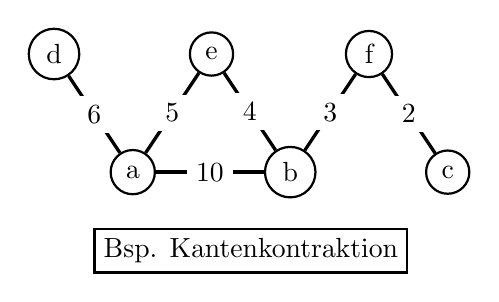
\begin{tikzpicture}{scale=0.8}
\begin{scope}[every node/.style={circle,thick,draw}]
    \node (d) at (0,0) {d};
    \node (e) at (2,0) {e};
    \node (f) at (4,0) {f};
    \node (a) at (1,-1.5) {a};
    \node (b) at (3,-1.5) {b};
    \node (c) at (5,-1.5) {c};
    \node [rectangle] (text) at (2.5,-2.5) {Bsp. Kantenkontraktion};
\end{scope}

\begin{scope}[>={Stealth[black]},
              every node/.style={fill=white},
              every edge/.style={draw=black,very thick}]
    \path [-] (d) edge node {$6$} (a);
    \path [-] (a) edge node {$5$} (e);
    \path [-] (e) edge node {$4$} (b);
    \path [-] (b) edge node {$3$} (f);
    \path [-] (f) edge node {$2$} (c);
    \path [-] (a) edge node {$10$} (b);
\end{scope}
\end{tikzpicture}
\end{center}
\end{halfboxl}%
\begin{halfboxr}
\vspace{-\baselineskip}
\begin{center}
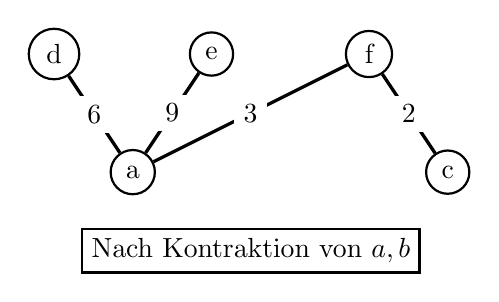
\begin{tikzpicture}{scale=0.8}
\begin{scope}[every node/.style={circle,thick,draw}]
    \node (d) at (0,0) {d};
    \node (e) at (2,0) {e};
    \node (f) at (4,0) {f};
    \node (a) at (1,-1.5) {a};
    \node (c) at (5,-1.5) {c};
    \node [rectangle] (text) at (2.5,-2.5) {Nach Kontraktion von $\Set{a,b}$};
\end{scope}

\begin{scope}[>={Stealth[black]},
              every node/.style={fill=white},
              every edge/.style={draw=black,very thick}]
    \path [-] (d) edge node {$6$} (a);
    \path [-] (a) edge node {$9$} (e);
    \path [-] (a) edge node {$3$} (f);
    \path [-] (f) edge node {$2$} (c);
\end{scope}
\end{tikzpicture}
\end{center}
\end{halfboxr}




\begin{halfboxl}
\vspace{-\baselineskip}
Der Algorithmus von Karger geht sehr einfach vor. Er erstellt für jeden Knoten eine Menge die ihn selbst enthält; werden zwei Knoten durch Kantenkontraktion fusioniert werden diese Mengen zusammengeführt, bis nur noch zwei Knoten vorhanden sind.

Dann wird die Knotenmenge des einen Knoten ausgegeben.

Da eine Kontraktion eine Laufzeit von $\mathcal{O}(n)$ hat, und in jeder Kontraktion einen Knoten abarbeitet, ergibt sich für den Algorithmus von Karger eine Laufzeit von $\mathcal{O}(n^2)$.
\end{halfboxl}%
\begin{halfboxr}
\vspace{-\baselineskip}
\begin{algo}{Algorithmus von Karger}
\textbf{Eingabe:} Ein Graph $G=(V,E,c)$.

\textbf{Ausgabe:} Ein Schnitt $S(v)$.
\tcblower
\begin{enumerate}
    \item Wir definieren $\Forall v S(v) := \Set{v}$ und $H := G$.
    \item Solange $|V(H)| > 2$ wähle beliebige Kante $\Set{v,w} \in V(H)$.
    \begin{enumerate}
        \item Setze $S(v) = S(v) \cup S(w)$ und kontraktiere $\Set{v,w}$ in $H$.
        \item Gebe $S(v)$ für eines der $v \in V(H)$ aus.
    \end{enumerate}
\end{enumerate}
\end{algo}
\end{halfboxr}
\begin{theo}{Erfolgswahrscheinlichkeit des Schnitts}
    $ P(C \text{ ist ein Min-Cut von } G) \ge \binom{n}{2}^{-1} $.
\end{theo}

\mrhere{fastcut-ewkeit}

Lassen wir diesen Algorithmus nun $t \cdot\binom{n}{2}$ Mal laufen (wobei wir $t \in \mathbb{N}$ frei wählen), so ist die Wahrscheinlichkeit den Min-Cut nicht zu finden $$\bigg( 1 - \binom{n}{2}^{-1} \bigg)^{t \cdot \binom{n}{2}} \le \bigg(\frac{1}{e}\bigg)^t.$$
Heißt, wir können die Fehlerwahrscheinlichkeit beliebig klein machen und so unsere Laufzeit töten, die mittlerweile wegen dem $\binom{n}{2}$ schon $\mathcal{O}(n^4)$ beträgt; und mal ganz ehrlich, das ist keine Verbesserung gegenüber herkömmlichen Algorithmen.

Aber die Wahrscheinlichkeit, eine Kante des Min-Cuts wegzukontraktieren, ist am Anfang des Algorithmus
relativ gering und steigt, sobald die Anzahl der Kanten sich zu sehr verringert. Die Idee wäre also den Algorithmus so zu verändern, dass wir am Anfang schnell Kanten kontraktieren und die letzten Schritte sicher machen.


\begin{halfboxl}
Das ist der Gedanke des Algorithmus von Karger und Stein, auch FastCut genannt. Dieser wird mit einem beliebigen Graph aufgerufen. Auf zwei Instanzen dieses Graphs werden rekursiv $t = \lceil 1 + \frac{n}{\sqrt{2}}\rceil$ Kanten kontraktiert, bis nur noch höchstens $c$ (oft mit $c = 6$) Kanten übrig sind. Von da an wird mit Brute-Force der Min-Cut bestimmt. Danach wird der kleinere Schnitt ausgegeben.

Das verbessert maßgeblich unsere Laufzeit.

\begin{theo}{Laufzeit von Karger und Stein}
Der FastCut Algorithmus hat eine Laufzeit von $\mathcal{O}(n^2\cdot \text{log }n)$
\end{theo}
\end{halfboxl}%
\begin{halfboxr}
\vspace{-\baselineskip}
\begin{algo}{Algorithmus von Karger und Stein (FastCut)}
\textbf{Eingabe:} Ein Graph $G=(V,E,c)$.

\textbf{Ausgabe:} Ein Schnitt $C_x$.
\tcblower
\begin{enumerate}

    \item Gilt $|V(G)| \le 6$, bestimme $C_U$ mit Brute-Force.
    \item Setze $H := H' := G$ und $t = \lceil 1+ \frac{n}{\sqrt{2}} \rceil$
    \item Kontraktiere Kanten bis in $H$ und $H'$ jeweils nur noch $t$ Kanten sind.
    \item Rufe FastCut rekursiv mit $C = \text{FastCut}(H)$ und $C'= \text{Fastcut}(H')$
    \item Gebe $\text{min}(C,C')$ aus.
\end{enumerate}
\end{algo}
\end{halfboxr}

Beweisideen:
\begin{itemize}
    \item Es gilt $T(n) = 2 \cdot T(\lceil 1 + \frac{n}{\sqrt{2}}\rceil) + \mathcal{O}(n^2)$ für $n > 6$ und  $T(n) = \mathcal{O}(1)$ für $n \le 6$.
    \item Wegen des konstanten Faktors $\frac{1}{\sqrt{2}}$ haben wir eine Rekursionstiefe von $D = \mathcal{O}(\text{log }n)$.
    \item Wir definieren uns $n_I$ die Menge der Knoten auf Rekursionstiefe $I$.
    \item Auf Rekursionstiefe $I$ lösen wir $2^I$ Teilproblem der Größe $n_I \equiv \frac{n}{\sqrt{2}^I}$.
    \item Dieses Teilproblem hat Laufzeit $\mathcal{O}(n_I^2)=\mathcal{O}(\frac{n^2}{2^I})$, auf einem Level also $2^I \cdot \mathcal{O}(\frac{n^2}{2^I}) = \mathcal{O}(n^2)$.
    \item Das multipliziert man mit der Rekursionstiefe für eine Laufzeit von $\mathcal{O}(n^2 \cdot \text{log } n)$.
\end{itemize}

\begin{theo}{Zuverlässigkeit von FastCut}
    FastCut berechnet den Min-Cut mit einer Wahrscheinlichkeit von $\Omega(\frac{1}{\text{log } n})$.
\end{theo}

\mrhere{fastcut}

\subsection{3-SAT}

\begin{defi}{3-SAT}
\textbf{Eingabe:}
\begin{itemize}
    \item Eine Boolsche Formel $\mathcal{F}$ in 3-KNF $\mathcal{F}(x_1,\ldots,x_n) = \bigwedge _{i=1}^m c_i$,
    \item bestehend aus Klauseln $\Forall i \in \underline{m}: c_i = (l_i^1 \lor l_i^2 \lor l_i^3)$,
    \item wiederum bestehend aus Literalen:
    \[\Forall i \in \underline{m} \quad \Forall j \in \underline{3}: \quad l_i^j = \begin{cases}
    \neg x_p & \text{oder} \\
    x_p & \text{für ein } p \in \underline{n}
    \end{cases} \]
\end{itemize}

\textbf{Ausgabe:} Eine Belegung $W: \Set{x_1,\ldots,x_n} \to \Set{0,1}$

\textbf{Ziel:} Finde eine erfüllende Belegung für $\mathcal{F}$.
\end{defi}

\begin{theo}{3-SAT}
    Für eine 3-KNF Formel zu bestimmen ob eine passende Belegung existiert ist NP-vollständig.
\end{theo}

Das Problem wollen wir aber sinnvoll angehen und lösen. Die Idee dabei ist, eine Belegung zu raten, ähnliche Lösungen im Lösungsraum zu betrachten und ansonsten eine neue Belegung testen.

\begin{algo}{Algorithmus von Schöning}
    \textbf{Eingabe:} Eine Boolsche Formel $\mathcal{F}(x_1,\ldots,x_n)$ in 3-KNF. \\
\textbf{Ausgabe:} Eine erfüllende Belegung $W : \Set{x_1,\ldots,x_n}\to \Set{0,1}$ oder eine Fehlermeldung.
\tcblower
\begin{enumerate}
    \item Wiederhole höchstens $\lceil 20 \cdot \sqrt{3 \cdot \pi \cdot n} \cdot \big(\frac{4}{3} \big)^n\rceil$ mal:
    \begin{enumerate}
        \item Rate eine zufällige Belegung $W = (w_1,\ldots,w_n) \in \Set{0,1}^n $, falls sie passt, gebe sie aus.
        \item Ansonsten führe maximal $3n$ mal aus:
        \begin{enumerate}
            \item Wähle beliebige Klausel und daraus beliebiges Literal.
            \item Kehre dieses Literal $w_j$ um. Falls $\mathcal{F}$ erfüllt ist, gebe $W = (w_1,\ldots,\neg w_j,\ldots,w_n)$ aus.
        \end{enumerate}
    \end{enumerate}
    \item Sonst terminiere und gebe aus, dass $\mathcal{F}$ nicht erfüllbar ist.
\end{enumerate}
\end{algo}

\begin{halfboxl}
\vspace{-\baselineskip}
\begin{theo}{Laufzeit von Schöning}
    Der Algorithmus von Schöning hat eine Laufzeit von $\mathcal{O}(m \cdot n^{3/2} \cdot \big(\frac{4}{3}\big)^n)$. Es können nur false negatives auftreten.
\end{theo}

\end{halfboxl}%
\begin{halfboxr}
\vspace{-\baselineskip}
\begin{theo}{Fehlerwahrscheinlichkeit von Schöning}
    Falls $\mathcal{F}$ erfüllbar ist, ist die Fehlerwahrscheinlichkeit $5 \cdot 10^{-5}$.
\end{theo}
\end{halfboxr}

Eine Belegung zu testen benötigt Laufzeit $\mathcal{O}(3m)$. Angesichts der Schleifen ist die Laufzeit des Algorithmus von Schöning relativ schnell ersichtlich.

Beweisideen der Fehlerwahrscheinlichkeit:

\begin{itemize}
    \item Für eine passende Belegung $W^*$ definieren wir Belegungsklassen, die der Anzahl der differierenden Bits $j$ entsprechen.
    \item In der Klasse $j$ zu landen hat eine Wahrscheinlichkeit von $p_j = \binom{n}{j}\cdot 2^{-n}$.
    \item Mit einer Mindestwahrscheinlichkeit von $\frac{1}{3}$ verbessern wir uns um eine Klasse. Umgekehrt ist die Verschlechterungswahrscheinlichkeit höchstens $\frac{2}{3}$.
    \item Die Wahrscheinlichkeit, um in $j + 2i \le 3n$ Schritten nach $W^*$ zu kommen ist
    $$q_{j,i}= \binom{j + 2i}{i} \cdot \frac{j}{j+2i}\cdot \bigg(\frac{1}{3}\bigg)^{j+i} \cdot \bigg(\frac{2}{3}\bigg)^{i}.$$
    \item Es ergibt sich für das Erreichen von $W^*$ aus $j$, die Summe über alle $i$: $$q_j = \frac{1}{2\cdot \sqrt{3\pi j}}\cdot \bigg(\frac{1}{2}\bigg)^j.$$
    \item Summieren wir über alle $j$ und runden das ganze schlau, erhalten wir für das Erreichen von $W^*$:
    $$\Tilde{p} = \frac{1}{2 \cdot \sqrt{3 \pi n}} \cdot \bigg(\frac{3}{4}\bigg)^n.$$
    \item Die Fehlerwahrscheinlichkeit ist dann nach $t = \lceil 20 \cdot \sqrt{3\pi n} \big(\frac{4}{3}\big)^n \rceil$ lokalen Suchen:
    $$(1- \Tilde{p})^t \le e^{\Tilde{p}t}= e^{-10} \le 5 \cdot 10^{-5}.$$
\end{itemize}

\subsection{Vergleich}

Randomisierte Algorithmen lassen sich in zwei Kategorien einteilen, nämlich einerseits Las Vegas Algorithmen und andererseits Monte-Carlo Algorithmen.

\begin{halfboxl}
\vspace{-\baselineskip}
\begin{defi}{Las Vegas Algorithmus $\mathcal{A}$}
\begin{itemize}
    \item $\mathcal{A}$ liefert immer eine optimale Lösung.
    \item Die Laufzeit hängt von Zufallvariablen ab.
\end{itemize}
\end{defi}
\end{halfboxl}%
\begin{halfboxr}
\vspace{-\baselineskip}
\begin{defi}{Monte-Carlo Algorithmus $\mathcal{B}$}
\begin{itemize}
    \item $\mathcal{B}$ liefert eine Lösung, die nur eventuell optimal ist.
    \item Die Lösung hängt nicht unbedingt von Zufallsvariablen ab.
\end{itemize}
\end{defi}
\end{halfboxr}

Die Algorithmen, die wir im Laufe des Kapitels behandelt haben, sind allesamt Monte-Carlo Algorithmen. Es ist aber möglich, Las Vegas und Monte-Carlo Algorithmen aufeinander zu reduzieren.

\begin{theo}{Las Vegas $\leftrightarrow$ Monte-Carlo}
Las Vegas und Monte-Carlo Algorithmen können aufeinander reduziert werden.
\end{theo}

Ideen (Las Vegas $\mathcal{A}$ $\to$ Monte-Carlo $\mathcal{B}$):
\begin{itemize}
    \item Hat $\mathcal{A}$ erwartete Laufzeit $f(n)$, brechen wir nach $\alpha \cdot f(n), 0 < \alpha < 1$ ab.
    \item Ergebnis ist eine Monte-Carlo Algorithmus $\mathcal{B}$ mit Fehlerwahrscheinlichkeit $\frac{1}{\alpha}$.
\end{itemize}

Ideen (Monte-Carlo $\mathcal{B}$ $\to$ Las Vegas $\mathcal{A}$):
\begin{itemize}
    \item Habe $\mathcal{B}$ eine Laufzeit von $f(n)$ mit Wahrscheinlichkeit $p(n)$ und sei $\mathcal{C}$ eine Routine, die in $g(n)$ die Korrektheit von $\mathcal{B}$ prüft.
    \item Wir lassen $\mathcal{A}$ so lange $\mathcal{B}$ und $\mathcal{C}$ aufrufen, bis $\mathcal{C}$ die Korrektheit bestätigt.
    \item Ergebnis ist ein Las Vegas Algorithmus $\mathcal{A}$ mit erwarteter Laufzeit $\frac{f(n)+g(n)}{p(n)}$.
\end{itemize}

\newpage
\section{Online-Algorithmen}
Offline-Algorithmen bekommen die gesamte Eingabe und können darauf das Problem lösen. Online-Algorithmen bekommen die Eingabe in Stücken, wobei für jedes Stück sofort eine unwiederrufbare Entscheidung getroffen werden muss.

\begin{halfboxl}
\vspace{-\baselineskip}
    \begin{defi}{Online-Algorithmus}
        Sei $\rho=\rho_1,\rho_2, \dots,\rho_m$ die Eingabe für ein Problem $\Pi$.
        Ein Algorithmus $A$ ist ein Online-Algorithmus, wenn:
        \begin{itemize}[nosep]
            \item Im $i$-ten Schritt erfolgt die Eingabe $\rho_i$.
            \item $A$ gibt auf $\rho_{1 \dots i} = \rho_1, \rho_2, \dots, \rho_i$ eine Lösung für $\Pi$ an.
            \item $A$ darf die Entscheidung auf $\rho_{1 \dots i-1}$ nicht verändern.
        \end{itemize}
    \end{defi}
\end{halfboxl}%
\begin{halfboxr}
\vspace{-\baselineskip}
    \begin{defi}{c-competitive}
        Sei $C_A(\rho)$ die Kosten der von $A$ berechneten Strategie auf der Eingabe $\rho$ und $C^*(p)$ die Kosten für die optimale Strategie. Dann ist $A$ $\textit{c-competitive}$ gdw. ein $a$ existiert, so dass für jede Eingabe $\rho$ gilt: $$C_A(\rho) \leq c \cdot C^*(\rho)+a.$$
    \end{defi}
\end{halfboxr}

\subsection{File-Allocation-Problem}
\begin{halfboxl}
Bei dem File-Allocation-Problem (FAP) gibt es mehrere Kopien einer Datei, die von mehreren Nutzern gelesen und beschrieben werden können. Die \emph{Migration} zwischen verschiedenen Speicherorten erzeugt {Kosten}. Für dieses Problem möchten wir einen guten Online-Algorithmus entwickeln.

Dazu betrachten wir ein System mit zwei Rechnern $a,b$ mit dem folgende Konfigurationen möglich ist: Die Datei ist nur auf $a$: [a], nur auf $b$: [b] oder auf $a$ und $b$: [a,b].

Die Eingabesequenz $\rho$ besteht aus Lese- und Schreibanfragen auf den Knoten.

Je nach Aktualität der Daten muss eventuell nachgeladen werden.
\end{halfboxl}%
\begin{halfboxr}
\vspace{-\baselineskip}
    \begin{defi}{File-Allocation-Problem}
        \textbf{Eingabe:} Eingabesequenz $\rho = \rho_1,\ldots,\rho_m$ mit Anfragen
            \begin{itemize}
                \item $\rho_i=r(v)$: Knoten $v \in \{a,b\}$ will Datei lesen.
                \item $\rho_i=w(v)$: Knoten $v \in \{a,b\}$ will Datei schreiben.
            \end{itemize}

        \textbf{Ausgabe:} Sequenz von Übergängen der Form
            \begin{itemize}
                \item $[v] \to [a,b]$, $[a,b] \to [v]$
                \item für $v,u \in \Set{a,b}$
            \end{itemize}

        \textbf{Ziel:} Minimiere entstehende \hyperref[subsubsec:fap-kosten]{Kosten}.
    \end{defi}
\end{halfboxr}

\subsubsection{Kosten}
\label{subsubsec:fap-kosten}
Es entstehen je nach Änderung der Konfiguration \emph{Service- und Migrationskosten}.   \\
Sei $v \in \{a,b\}$, dann entstehen Servicekosten von einer Einheit...
\begin{itemize}
    \item beim Lesen: Anfrage $\rho_i=r(v)$ in Konfiguration $[u]$, mit $u \in \{a,b\} \setminus \{v\}$
    \item beim Schreiben: Anfrage $\rho_i=w(v)$ in Konfiguration $[a,b]$ oder $[u]$, mit $u \in \{a,b\} \setminus \{v\}$
\end{itemize}
Migrationskosten von $1$ enstehen, wenn die Konfiguration geändert wird, aber nicht beim Löschen. Etwa wenn die Datei von einem auf beide Leser kopiert wird.

Wenn wir einen konstanten competitiven Faktor wollen, müssen wir intelligent migrieren:
\begin{itemize}
    \item Von $[a,b]$ nach $[x]$, falls eine Anfrage $w(x)$ mit $x \in \{a,b\}$.
    \item Von $[a]$ nach $[b]$ oder $[a,b]$, falls eine Anfrage $r(b)$ erfolgt.
    \item Von $[b]$ nach $[a]$ oder $[a,b]$, falls eine Anfrage $r(a)$ erfolgt.
\end{itemize}
Die Konfiguration $[a,b]$ ist scheinbar zu bevorzugen.

\begin{theo}{Obere und Untere Schranke}
    \begin{enumerate}
        \item Für das uniforme FAP auf zwei Knoten gibt es einen $3$-kompetitiven Online-Algorithmus.
        \item Für das uniforme FAP auf zwei Knoten gibt es keinen $c$-kompetitiven Online-Algorithmus mit $c < 3$.
    \end{enumerate}
\end{theo}

\subsubsection{Obere Schranke}

\begin{halfboxl}
Im Folgenden zeigen wir einen Online-Algorithmus, der $3$-competitive ist.

Die initialen Kosten sind einmalig, und erhöhen den competitiven Faktor nicht.

Fall 1: Tritt auf, wenn eine Lese- oder Schreibanfrage an einen Knoten ohne Datei kommt. Es entstehen je eine Kosteneinheit für die Anfrage und die Migration, also Kosten von $2$.

Fall 2: Tritt auf, wenn eine Schreibanfrage an einen der Knoten kommt und beide die Datei aktuell hatten. Es entstehen Kosten von $1$ für die Anfrage, da Löschen nichts kostet.
\end{halfboxl}%
\begin{halfboxr}
\vspace{-\baselineskip}
\begin{algo}{Online-Algorithmus zu FAP}
    \textbf{Eingabe:} Lese- und Schreibanfragen.

    \textbf{Ausgabe:} Änderung der optimalen Konfiguration nach jedem Schritt.
    \tcblower
    Initial gehe in die Kofiguration $[a,b]$.

    Danach unterscheide zwei Fälle:
    \begin{itemize}
        \item Falls in der Konfiguration $[x]$ eine Anfrage $\rho_i \in \{r(v),w(v)\}$ mit $x \neq v$ kommt, gehe in die Konfiguration $[a,b]$.
        \item Falls in der Konfiguration $[a,b]$ eine Anfrage $\rho_i=w(v)$ kommt, gehe in die Konfiguration $[v]$.
    \end{itemize}
\end{algo}
\end{halfboxr}

Wir zeigen, dass das obige Verfahren $3$-competitive ist.
Im Folgenden sei dazu $x \in \{a,b\}$.

Wir starten in der Konfiguration $[a,b]$. Diese Konfiguration ändert sich erst nach dem ersten Schreibzugriff in $[a]$ oder $[b]$. O.B.d.A. gehen wir in die Konfiguration $[a]$. Von da aus gibt es nur einen möglichen Konfigurationswechsel auf $[a,b]$, ausgelöst durch Lesen oder Schreiben auf $b$. Es gibt also keine direkten Übergänge von $[a]$ auf $[b]$ oder umgekehrt, sondern nur von $[x]$ auf $[a,b]$ und von $[a,b]$ auf $[x]$.

Wir teilen die Anfragesequenz in disjunkte \emph{Phasen} maximaler Länge auf. Die Zugriffe einer Phase enden dabei immer in der gleichen Kofiguration. Die ersten Kosten enstehen erst bei dem ersten Schreibzugriff der auf $[x]$ endet. O.B.d.A. nehmen wir deshalb an, dass die Sequenz mit einer $[x]$-Phase beginnt. Danach folgt eine $[a,b]$-Phase und diese wechseln sich dann ab.

Wir führen eine \emph{Doppelphase} ein, die aus einer $[x]$-Phase und einer $[a,b]$-Phase besteht. Die Online-Sequenz besteht somit aus disjunkten aneinander gereihten Doppelphasen.

Wir zeigen nun, dass eine Doppelphase Kosten $3$ hat. Am Anfang einer Doppelphase entstehen Servicekosten von $1$ durch den Schreibzugriff auf $x$. Alle folgenden Zugriffe in der $[x]$-Phase erzeugen keine Kosten. Erst der erste Zugriff in der $[a,b]$-Phase hat Servicekosten und Migrationskosten, also insgesamt Kosten von $2$. Alle weiteren Anfragen in dieser Phase verursachen keine Kosten. Insegsamt sind das Kosten von $3$ pro Doppelphase.

Jetzt zeigen wir, dass jeder andere Algorithmus Kosten von mindestens $1$ in einer Doppelphase hat. Angenommen $A$ sei ein Algorithmus mit Kosten $0$ in einer Doppelphase. Dann muss die Konfiguration zu Beginn $[x]$ sein, da die Phasen mit einem Schreibzugriff beginnen und sonst schon Kosten entstehen würden. Weiterhin kann $A$ diese Konfiguration $[x]$ nicht verlassen, da sonst Migrationskosten entstehen. Da aber der Beginn einer $[a,b]$-Phase von dem anderen Knoten initiiert wird, müssen doch Kosten entstehen. Also hat $A$ mindestens Kosten $1$ pro Doppelphase.

Damit ist gezeigt, dass unser Online-Algorithmus $3$-competitive ist.

\subsubsection{Untere Schranke}

Wir zeigen nun, dass kein Algorithmus competitive-Faktor kleiner $3$ hat.

Dazu zeigen wir für einen beliebigen Algorithmus $A$, dass es eine Eingabe und $3$ andere Algorithmen gibt, die auf der Eingabe zusammen die selben Kosten wie $A$ verursachen.

Diese Eingabe wird nur aus Schreibzugriffen bestehen. Auf solchen kann der Algorithmus die Kosten nicht verringern, indem er die Konfiguration $[a,b]$ nutzt. Also nehmen wir o.B.d.A.\ an, dass diese nicht verwendet wird.

Dann sei die Eingabe so, dass wenn der Algorithmus nach den ersten $i$ Eingaben in Konfiguration $[x]$ ist, als nächstes Zugriff $w(y)$ mit $x \ne y$ kommt.

Auf der selben Eingabe betrachten wir diese anderen Algorithmen:
\begin{itemize}
    \item $B$, der stets das Gegenteil von $A$ macht. Das heißt, wenn $A$ in Konfiguration $[x]$ übergeht, geht $B$ in Konfiguration $[y]$ mit $y \ne x$ über.
    \item $C_A$, der stets in Konfiguration $[a]$ verbleibt.
    \item $C_B$, der stets in Konfiguration $[b]$ verbleibt.
\end{itemize}

Dann hat $B$ genau dann Migrationskosten, wenn $A$ Migrationskosten hat, aber auf dieser Eingabe nie Servicekosten. $C_A$ und $C_B$ haben nie Migrationskosten, aber in jedem Schritt hat genau einer von beiden Servicekosten.

Also sind die Gesamtkosten von $A$ die Summe der Kosten dieser Algorithmen. Da der optimale Algorithmus nicht schlechter sein kann, kann $A$ keinen competitive-Faktor kleiner $3$ haben.

\subsection{Paging-Problem}
Wir betrachten ein zweischichtiges Speichersystem: Ein großer, langsamer \emph{Hauptspeicher} und ein schneller \emph{Cache} mit Platz für $k$ Seiten. Dazu gibt es \emph{Anfragen} $t$ an den Speicher, die genau einer Seite entsprechen. Falls $t$ nicht im Cache ist (\textit{Seitenfehler}) so muss diese Seite \emph{nachgeladen werden}. Falls der Cache voll ist, muss eine Seite \emph{verdrängt} werden.

\subsubsection{Deterministisch}
Dazu gibt es verschieden \emph{deterministische} Strategien:
\begin{itemize}
    \item \textit{LRU} (Least Recently Used): Verdrängte die Seite, deren letzter Zugriff am längsten zurückliegt.
    \item \textit{LFU} (Last Frequently Used): Verdrängt die am seltensten nachgefragte Seite.
    \item \textit{FIFO} (First In First Out): Verdrängt die Seite, die sich am längsten im Cache befindet.
    \item \textit{LIFO} (Last In First Out): Verdrängt die Seite, die als letztes in den Cache geladen wurde.
    \item \textit{RANDOM}: Verdrängt eine Uniform ausgewählte Seite.
    \item \textit{FWF} (Flush When Full): Leert den Cache vollständig, sobald eine Seite verdrängt werden muss.
    \item \textit{LFD} (Longest Forward Distance): Verdrängt die Seite, deren Zugriff am weitesten in der Zukunft liegt.
\end{itemize}
$\textit{LFD}$ ist das \emph{optimale} Verfahren, aber kein Online-Algorithmus.

Um den \emph{competitiven} Faktor eines Paging Verfahrens zu bestimmen, müssen wir Seitenauslagerungen erkennen. Dazu führen wir ein Marking ein.

\begin{halfboxl}
    \textit{Marking:} Da jedes Verfahren bei $k+1$ verschiedenen Seitenzugriffen mindestens einen Fehler macht, teilen wir die Eingabesequenz in Phasen mit Zugriffen auf $k$ verschiedene Seiten, d.h.\ die nächste Phase startet beim Zugriff auf die $k+1$-te neue Seite.

    In einer Phase wird jede Seite beim erstmaligen Zugriff \textit{markiert} und bleibt bis zum Ende der Phase markiert.

    Damit können wir die Verfahren in zwei Klassen aufteilen: Verfahren, die nie eine markierte Seite verdrängen und solche, die auch Markierte verdrängen.
\end{halfboxl}%
\begin{halfboxr}
\vspace{-\baselineskip}
    \begin{defi}{Marking-Algorithmus}
        Ein \emph{Marking-Algorithmus} verdrängt niemals eine markierte Seite.

        Eine \emph{markierte Seite} ist eine Seite, auf die in der aktuellen Phase schon zugegriffen wurde.

        In einer \emph{Phase} wird auf $k$ verschiedenen Seiten zugegriffen.
    \end{defi}
\end{halfboxr}

\textit{LRU} und \textit{FWF} sind Marking-Algorithmen.

\begin{halfboxl}
    \textit{Beweis ($LRU$):} Betrachte eine beliebige Phase $P_i$, in der höchstens $k$ Seiten markiert sind. Auf jeder der markierten Seiten ist in $P_i$ zugegriffen worden, sodass $LRU$ diese Seiten in dieser Phase nicht verdrängt.
\end{halfboxl}%
\begin{halfboxr}
\vspace{-\baselineskip}
    \textit{Beweis ($FWF$):} $FWF$ entleert den Cache erst, wenn eine Seite verdrängt werden muss, also nach mehr als $k$ verschiedenen Seitenzugriffen und genau am Ende einer Phase. Damit ist $FWF$ Marking-Algorithmus.
\end{halfboxr}

Wir beweisen, dass jeder Marking-Algorithmus $k$-competitive ist: Zu jeder Zeit sind alle markierten Seiten im Cache.
\begin{itemize}
    \item Jede neue Markierung verursacht höchstens einen Seitenfehler.
    \item Damit gibt es pro Phase höchstens $k$ Seitenfehler.
    \item Außerdem muss jeder Paging-Algorithmus mindestens eine Seite pro Phase verdrängen.
\end{itemize}
Also sind Marking-Algorithmen $k$-competitive.  \\
\mrhere{marking-comp}

Damit sind auch $FWF$ und $LRU$ $k$-competitive.

\begin{halfboxl}
\vspace{-\baselineskip}
    \begin{theo}{FIFO}
        \textit{FIFO} ist kein Marking-Algorithmus, aber $k$-competitive.
    \end{theo}
\end{halfboxl}%
\begin{halfboxr}
\vspace{-\baselineskip}
    \begin{theo}{LIFO}
        \textit{LIFO} ist nicht $c$-competitive für beliebiges $c \in \mathbb{R}$.
    \end{theo}
\end{halfboxr}

\begin{halfboxl}
\vspace{-\baselineskip}
    \begin{theo}{LFU}
        $LFU$ ist nicht $c$-competitive für beliebiges $c \in \mathbb{R}$.
    \end{theo}
\end{halfboxl}%
\begin{halfboxr}
    \vspace{-\baselineskip}
    \begin{proof}
    Mit der Eingabesequenz \\$\rho=p_1^{m},p_2^{m},\dots,p_{k-1}^{m},(p_k,p_{k+1})^{m-1}$ werden nach $m \cdot (k-1)$ Zugriffen $2(m-1)$ viele Fehler erzeugt. Mittels $m$ kann man den Competitive-Faktor beliebig verschlechtern.
    \end{proof}
\end{halfboxr}

\subsubsection{Untere Schranke}
Wir beweisen nun, dass deterministische Verfahren nur begrenzt gut sein können.

\begin{theo}{Untere Schranke}
    Es gibt keinen deterministischen Online-Algorithmus für das Paging-Problem mit competitive-Faktor besser als $k$.
\end{theo}

Um dies zu beweisen, vergleichen wir einen Online-Algorithmus $A$ mit einem optimalen Offline-Algorithmus $B$. Sei der Hauptspeicher beider Algorithmen $k+1$ Seiten und der Cache jeweils $k$ Seiten groß.

Fülle nun beide Caches mit den gleichen $k$ Seiten. Jetzt wird die Eingabesequenz so gewählt, dass $A$ immer die Seite nachlädt, die nicht im Cache ist, sondern als einzige nur im Hauptspeicher liegt. $B$ dagegen lagert diejenige Seite aus, die mindestens in den nächsten $k-1$ Schritten nicht angefragt wird.

Bevor beide den Seitenfehler machen, müssen sie die selben Seiten im Cache haben. Also kann man dies unbeschränkt fortführen. Dann macht $A$ bei einer Sequenz mit Länge $k+m$ auch $k+m$ Seitenfehler, $B$ macht aber bei $k+m$ Anfragen höchstens $k+\ceil*{\frac{m}{k}}$ Seitenfehler.

\subsubsection{Random}
Da wir gesehen haben, dass deterministische Paging-Algorithmen höchstens k-competitive sind und der ``Gegner'' eine unvorteilhafte Sequenz wählen kann, schauen wir uns jetzt \emph{randomisierte} Online-Algorithmen an.

Dabei wird der Zufallsanteil erst nach dem Wählen der Sequenz genutzt. Wir nennen den Algorithmus, oder Gegner, der die Eingabe erstellt, \emph{oblivious} (blind, vergesslich).

\begin{defi}{c-competitive für Random}
    Ein randomisierter Online-Algorithmus $A$ ist c-competitive gdw. ein $a$ existiert, so dass für jede durch einen oblivous Gegner bestimmte Anfragesequenz $\rho$ gilt: $$\mathbb{E}[C_A(\rho)] \leq c \cdot C^*(\rho)+a.$$
\end{defi}

Dazu gibt es einen einfachen randomisierten Online-Algorithmus.

\begin{halfboxl}
\vspace{-\baselineskip}
    \begin{algo}{MARK}
        \textbf{Eingabe:} Cache mit $k$ vollen Seiten.

        \textbf{Ausgabe:} Cache mit $k-1$ vollen Seiten.
        \tcblower
        Für jeden Seitenfehler pro Phase:
        \begin{enumerate}
            \item Bestimme unmarkierte Seiten
            \item Verdränge eine uniform gewählte unmarierte Seite
        \end{enumerate}
    \end{algo}
\end{halfboxl}%
\begin{halfboxr}
\vspace{-\baselineskip}
    \begin{theo}{Schranke $H_k$-competitive}
        Es gibt einen anderen Paging-Algorithmus, der $H_k$-competitive ist, aber keinen der besser als $H_k$-competitive ist.
    \end{theo}
\end{halfboxr}

In der Vorlesung wurde außerdem bewiesen, dass $MARK$ $(2 \cdot H_k)$-competitive ist.

Der Beweis wird hier aufgrund seiner Länge nicht erklärt.

\subsubsection{Asymmetrischer Online-Algorithmus}
\begin{halfboxl}
Da der Offline-Algorithmus die gesamte Eingabe kennt, hat er einen unfairen Vorteil. Wir geben dem Online-Algorithmus daher mehr Cache.

Der Online-Algorithmus bekommt einen Cache der Größe $m \cdot k$, wenn der Offline-Algorithmus einen Cache der Größe $k$ hat. Ein solcher Unterschied in den Einschränkungen an die Algorithmen nennt man \emph{Asymmetrie}.
\end{halfboxl}%
\begin{halfboxr}
\vspace{-\baselineskip}
\begin{defi}{$(m,c)$-competitive}
    Ein Online-Algorithmus $A$ für das Paging-Problem ist $(m,c)-competitive$ gdw.
    \begin{itemize}
        \item $m$-mal so großer Cache wie Offline,
        \item es existiert ein $a$, sodass für jede Eingabesequenz $\rho$ gilt $C_A(\rho) \leq c \cdot C^*(\rho)+a$.
    \end{itemize}
\end{defi}
\end{halfboxr}

Wir beweisen nun, dass $Random$ $(2,2)$-competitive ist.

Dazu werden wir eine Potentialfunktion $\phi$ nutzen und zeigen, dass stets
\[\mathbb{E}[C] + 2\mathbb{E}[\phi] \le 2 C^\ast\]
ist, wobei $E[C]$ die erwarteten Kosten von $Random$ und $C^\ast$ die Kosten der optimalen Offline-Strategie sind.

Wir definieren $\phi$ als die Anzahl der Seiten, die im Cache von $OPT$ sind, aber nicht im Cache von $Random$. Dann kann $\phi$ nicht negativ sein, also reicht die obige Invariante, um den competitive-Faktor zu zeigen.

Die Invariante zeigen wir nun Schrittweise (deswegen auch die Potentialfunktion). Wir betrachten den Seitenzugriff auf eine Seite $p_t$ und unterscheiden viel Fälle:
\begin{enumerate}
    \item Beide Strategien haben $p_t$ bereits im Cache. Dann bleiben $C$, $\phi$ und $C^\ast$ gleich.
    \item Keine Strategie hat $p_t$ schon im Cache. Dann erhöhen sich $C$ und $C^\ast$ beide um $1$, $\mathbb{E}[\phi]$ erhöht sich höchstens um $\frac{1}{2}$, da die Wahrscheinlichkeit, dass $Random$ eine Seite verdrängt, die $OPT$ im Cache hält, höchstens $\frac{1}{2}$ ist.
    \item $Opt$ hat die Seite im Cache, aber $Random$ nicht. Dann bleibt $C^\ast$ gleich, $C$ erhöht sich um $1$ und $\mathbb{E}[\phi]$ verringert sich mindestens um $\frac{1}{2}$, da $Random$ sich um $p_t$ an $Opt$ angleicht und eine andere Seite, die $Opt$ im Cache hat, mit Wahrscheinlichkeit höchstens $\frac{1}{2}$ verdrängt.
    \item $Random$ hat die Seite im Cache, aber $Opt$ nicht. Dann erhöht sich $C^\ast$ um $1$, $C$ bleibt gleich und $\mathbb{E}[\phi]$ kann sich höchstens verringern.
\end{enumerate}
Also wird die Invariante in allen Fällen beibehalten. Da sie zu Beginn gilt, muss sie also immer gelten.

\label{ende}
\newpage
\section{Verständnisfragen}

\subsection*{Flussprobleme}

\begin{itemize}
    \item Was ist die Laufzeit der Ford-Fulkerson Methode?
    \item Wann hat die Ford-Fulkerson Methode die maximale Laufzeit?
    \item Warum liefert die Ford-Fulkerson Methode den maximalen Fluss?
    \item Was ist die Laufzeit der Ford-Fulkerson Methode mit Breitensuche?
    \item Wie ist die Idee des Min-Cut-Max-Flow Theorems?
    \item Wie wird der Schnitt zu dem maximalen Fluss gefunden?
    \item Was ist die Idee des Algorithmus von Dinitz?
    \item Wie funktioniert die Forward-Propagation?
    \item Wie ist die Laufzeit vom Algorithmus von Dinitz?
    \item Wie ist die Begründung zur Laufzeit vom Algorithmus von Dinitz?
    \item Wie bestimmt man Flüsse mit einem Mindestfluss auf den Kanten?
    \item Wie bestimmt man Flüsse mit einem Mindestfluss auf den Kanten, auf denen aber auch ein leerer Fluss erlaubt ist?
    \item Wie ist die Idee der Algorithmen zu kostenminimalen Flüssen?
    \item Was ist die Laufzeit der Algorithmen zu kostenminimalen Flüssen?
    \item Was ist die Idee zum Beweis der Laufzeit der Algorithmen zu kostenminimalen Flüssen?
\end{itemize}

\begin{halfboxl}

\subsection*{Matchings}
\begin{itemize}
    \item Wie kann man das bipartite Matching mit Flussalgorithmen lösen?
    \item Welche Laufzeiten haben die verschiedenen Matchingprobleme?
    \item Welcher Zusammenhang besteht zwischen verbessernden Pfaden und einem Maximum Matching?
    \item Wie ist die Vorgehensweise, um eine Laufzeit von $\bigo(m\sqrt{n})$ für das Matchingproblem zu erhalten?
    \item Wie ist die Vorgehensweise, um das Matching auf allgemeinen Graphen zu bestimmen?
\end{itemize}

\end{halfboxl}%
\begin{halfboxr}

\subsection*{Approximation}
Wie können die folgenden Probleme approximiert werden? Welche untere Schranke ist bekannt?
\begin{itemize}
    \item Cliquenproblem
    \item Färbungsproblem
    \item Vertex Cover
    \item Independent Set
    \item Steinerbaum Problem
    \item TSP
    \item $\Delta$-TSP
    \item Zentrumsproblem
    \item Set Cover
\end{itemize}

\end{halfboxr}

\begin{halfboxl}

\subsection*{Scheduling}
\begin{itemize}
    \item Wie arbeitet die LL Heuristik?
    \item Wie arbeitet die LPT Heuristik?
    \item Wie ist die Güte der LL Heuristik? Wie ist der Beweis?
    \item Wie ist die Güte der LPT Heuristik? Wie ist der Beweis?
    \item Wie arbeitet das Approximationsschema für Makespan Scheduling? Wie ist die Beweisidee?
    \item Wie kann des Makespan Problem auf allgemeinen Maschinen approximiert werden? Wie ist die Beweisidee?
\end{itemize}

\end{halfboxl}%
\begin{halfboxr}

\subsection*{Lineare Programmierung}
\begin{itemize}
    \item Wie ist die Idee der Simplexmethode?
    \item Welche Laufzeit erhalten wir bei der Simplexmethode?
    \item Wie ist die Idee der Ellipsoidmethode?
    \item Welche Laufzeit erhalten wir bei der Ellipsoidmethode?
    \item Wie arbeitet die Perturbierung?
    \item Wie arbeitet der Algorithmus von Seidel?
    \item Wie ist die Laufzeit für den Algorithmus von Seidel?
\end{itemize}

\end{halfboxr}

\begin{halfboxl}

\subsection*{Randomisierte Algorithmen}
\begin{itemize}
    \item Was ist ein Monte-Carlo-Algorithmus?
    \item Was ist ein Las-Vegas-Algorithmus?
    \item Wie können sich Monte-Carlo- und Las-Vegas-Algorithmen gegenseitig simulieren?
    \item Wie arbeitet der randomisierte Algorithmus für einen minimalen Schnitt?
    \item Wie ist die Laufzeit des randomisierten Algorithmus für einen minimalen Schnitt?
    \item Wie funktioniert der Algorithmus von Schöning?
    \item Wie ist die Fehlerwahrscheinlichkeit beim Algorithmus von Schöning?
\end{itemize}

\end{halfboxl}%
\begin{halfboxr}

\subsection*{Online-Algorithmen}
\begin{itemize}
    \item Wie arbeitet der Online-Algorithmus für das File Allocation-Problem?
    \item Wie ist die untere Schranke für jeden deterministischen Online-Algorithmus für das FAP?
    \item Welche Paging-Algorithmen gibt es?
    \item Was ist ein Marking-Algorithmus?
    \item Was ist der competitive Faktor von Marking Algorithmen?
    \item Was ist der competitive Faktor vom $LFU$ Algorithmus?
    \item Wie gut können deterministische Paging Algorithmen sein?
    \item Wie gut sind randomisierte Paging Algorithmen?
    \item Wie gut können asymmetrische Paging Algorithmen sein?
\end{itemize}

\end{halfboxr}

\newpage
\sffamily
\section{Wir wollen eure Merge Requests!}
\label{sec:merge-requests}
Trotz der~\pageref*{ende} Seiten, die wir schon haben, gibt es noch viel zu tun. Falls ihr euch damit quälen und gleichzeitig Anderen helfen wollt, sehen wir gerne Merge Requests zu beliebigen Themen, insbesondere aber zu den folgenden Stellen:
\begin{itemize}
    \item\label{mrExp:mean-algo} \hyperlink{mr:mean-algo}{Mean Algorithmus}   \\
    Von den beiden Laufzeitschranken wurde bisher nur eine erklärt.
    \item\label{mrExp:maximum-matching}\hyperlink{mr:maximum-matching}{Maximum Matching}  \\
    Der Beweis, dass der Greedy-Algorithmus eine 2-Approximation für Maximum Matching liefert, war mal in einer Übung. Den könnte man hier nochmal umreißen.
    \item\label{mrExp:set-cover}\hyperlink{mr:set-cover}{Set Cover}   \\
    Der Beweis des Approximationsfaktors fehlt.
    \item\label{mrExp:allgemeine-maschinen}\hyperlink{mr:allgemeine-maschinen}{Scheduling: Allgemeine Maschinen}  \\
    Leicht unvollständig.
    \item\label{mrExp:clique}\hyperlink{mr:clique}{Clique}    \\
    Nichtapproximierbarkeit könnte man noch besser erklären.
    \item\label{mrExp:lp-geo}\hyperlink{mr:lp-geo}{LP: Geometrische Lösung}    \\
    Könnte man hier eigentlich auch noch erklären.
    \item\label{mrExp:lp-simplex}\hyperlink{mr:lp-simplex}{LP: Simplex}   \\
    Die Laufzeitbeweise.
    \item\label{mrExp:lp-seidel-box}\hyperlink{mr:lp-seidel-box}{LP: Die Box-Bedingungen bei Seidel}  \\
    Das könnte man noch besser erklären.
    \item\label{mrExp:fastcut}\hyperlink{mr:fastcut}{Fastcut} \\
    Der Zuverlässigkeitsbeweis fehlt noch.
    \item\label{mrExp:min-weight-perfect-matching}\hyperlink{mr:min-weight-perfect-matching}{Minimum Weight Perfect Matching}    \\
    Wurde in der Übung Äquivalenz zu Max-Weight Matching gezeigt. Da das Problem beim \hyperref[algo:tsp-15-approx]{Algorithmus von Christofides} wieder auftaucht, könnte man das hier zumindest definieren.
    \item\label{mrExp:marking-comp}\hyperlink{mr:marking-comp}{Marking Algorithms}    \\
    Man könnte den competitive-Faktor noch besser begründen.
    \item\label{mrExp:fastcut-ewkeit}\hyperlink{mr:fastcut-ewkeit}{Fastcut: Erfolgswahrscheinlichkeit}    \\
    Die Ideen für die Erfolgswahrscheinlichkeit könnte man noch erklären.
\end{itemize}

\end{document}
